%% \documentclass[handout,t]{beamer} % HANDOUT
%% \documentclass[handout,notes=show,t]{beamer} % NOTES
\documentclass[t]{beamer} % SLIDES
\usepackage{etex}

\usetheme{DSM}
\usepackage{beamer-tools-dsm}

%%
%% some useful macros: mathematical notation etc.
%%

%% abbreviations for logic symbols
\renewcommand{\implies}{\Rightarrow}
\newcommand{\equivalent}{\Leftrightarrow}

%% abbreviations for common number spaces
\newcommand{\setN}[1][]{\mathbb{N}_{#1}} % allows \setN and \setN[0]
\newcommand{\setZ}{\mathbb{Z}}
\newcommand{\setQ}{\mathbb{Q}}
\newcommand{\setR}{\mathbb{R}}

%% sets and (sub-)sets defined by condition
\newcommand{\set}[1]{\{#1\}}
\newcommand{\setdef}[2]{\set{#1\,|\,#2}}
\newcommand{\bigset}[1]{\bigl\{#1\bigr\}}
\newcommand{\bigsetdef}[2]{\bigset{#1\bigm|#2}}
\newcommand{\setscale}[1]{\left\{#1\right\}}
\newcommand{\setdefscale}[2]{\setscale{#1\left|\,#2\right.}}

%% absolute value and norm
\newcommand{\abs}[1]{\lvert #1\rvert}
\newcommand{\bigabs}[1]{\bigl\lvert #1\bigr\rvert}
\newcommand{\absscale}[1]{\left\lvert #1\right\rvert}
\newcommand{\norm}[2][]{\lVert #2\rVert_{#1}}
\newcommand{\bignorm}[2][]{\bigl\lVert #2\bigr\rVert_{#1}}
\newcommand{\normscale}[2][]{\left\lVert #2\right\rVert_{#1}}

%% complement set (with optional index)
\newcommand{\compl}[1][]{\mathcal{C}^{#1}}

%% power set: \powerset{\Sigma^*}
\newcommand{\powerset}[1]{\mathcal{P}(#1)}

%% uparrow: a \ua b = direct dominance in ordered tree
\newcommand{\ua}{\uparrow}

%% left-right arrow: this $\lra$ that
\newcommand{\lra}{\leftrightarrow}

%% expanded engineering notation: 4.2\x\e+5
\newcommand{\e}[2]{10^{\ifthenelse{\equal{#1}{+}}{}{#1}#2}}
\newcommand{\x}{\cdot}

%% arg max & min: \argmax_{x\in C}, \argmin_{x\in C}
\newcommand{\argmax}{\mathop{\text{arg~max}}}
\newcommand{\argmin}{\mathop{\text{arg~min}}}

%% infinitesimal elements: \dx, \dy = \dX{y}, \dz
\newcommand{\dX}[1]{\,\mathit{d{#1}}}
\newcommand{\dx}{\dX{x}}
\newcommand{\dy}{\dX{y}}
\newcommand{\dz}{\dX{z}}

%%% Local Variables: 
%%% mode: latex
%%% TeX-master: ""
%%% End: 
  % basic mathematical notation
%%
%% some macros for typesetting text
%%

%% \OPEN ... \CLOSE; \OPEN[np] ... \CLOSE[np]
%% bold large brackets for labelled bracketing notation
\newcommand<>{\OPEN}[1][]{\only#2{$\boldsymbol{\bigl[}\text{}_{\text{\raisebox{-2pt}{\textsc{#1}}}}$}}
\newcommand<>{\CLOSE}[1][]{\only#2{$\text{}_{\text{\raisebox{-2pt}{\textsc{#1}}}}\boldsymbol{\bigr]}$}}

%% \textgap ("_" representing missing letter)
\newcommand{\textgap}{\mbox{\hspace{.4pt}\texttt{\bfseries\secondary{\textunderscore}}\hspace{.4pt}}}

%% \textstar, \textast (math \star and \ast symbols in text mode, with some extra spacing)
% \newcommand{\textstar}{$\mspace{.8mu}\star\mspace{.8mu}$}
% \newcommand{\textast}{$\ast$}

%% $\p{\ctext{abc}}$ (cited text in mathematical equations, e.g. n-gram probabilities)
\newcommand{\ctext}[1]{\text{\textcite{#1}}}

%% $\p{\btext{abc}}$ (normal black text even in coloured math environment)
\newcommand{\btext}[1]{\text{\foreground{#1}}} 

%% text subscripts and superscripts (can be used in math and text mode)
\newcommand{\tsup}[1]{\ensuremath{^{\text{#1}}}}
\newcommand{\tsub}[1]{\ensuremath{_{\text{#1}}}}

%%% Local Variables: 
%%% mode: latex
%%% TeX-master: ""
%%% End: 
  % some useful macros for plain text
%%
%% some useful macros: statistical notation
%%

%% \p{X=k};  \pC{X=k}{Y=l};  \bigp{X_i = k};   \pscale{\frac{Z}{S^2}};
%% probability P(X=k) and conditional probability P(X=k|Y=l), also with larger or scaled parentheses
%% \p[\theta]{X=k};  \pC[\text{interpolated}]{X=k}{Y=l};  ...
%% with optional subscripts (for model probability, null probability, etc.)
\newcommand{\p}[2][]{\mathop{\mathrm{Pr}_{#1}}(#2)}
\newcommand{\pscale}[2][]{\mathop{\mathrm{Pr}_{#1}}\!\left(#2\right)}
\newcommand{\bigp}[2][]{\mathop{\mathrm{Pr}_{#1}}\bigl(#2\bigr)}
\newcommand{\pC}[3][]{\p[#1]{#2\,|\,#3}} 
\newcommand{\pCscale}[3][]{\pscale[#1]{#2\left|\,#3\right.\!}} 
\newcommand{\bigpC}[3][]{\bigp[#1]{#2\!\bigm|\!#3}} 

%% \Exp{X};  \Var{X};  \Exp[0]{X};  \Var[0]{X};  
%% \bigExp{X}; \bigVar{X}; \Expscale{X};  \Varscale{X};
%% expectation E[X] and variance V[X], expectation and variance under null hypothesis, 
%% and variants with largeer or scaled brackets
\newcommand{\Exp}[2][]{\mathrm{E}_{#1}[#2]}
\newcommand{\Var}[2][]{\mathop{\mathrm{Var}}_{#1}[#2]}
\newcommand{\bigExp}[2][]{\mathrm{E}_{#1}\!\bigl[#2\bigr]}
\newcommand{\bigVar}[2][]{\mathop{\mathrm{Var}}_{#1}\bigl[#2\bigr]}
\newcommand{\Expscale}[2][]{\mathrm{E}_{#1}\left[#2\right]}
\newcommand{\Varscale}[2][]{\mathop{\mathrm{Var}}_{#1}\left[#2\right]}

%% \pihat = \hat{\pi}
%% sampling estimate for population probability \pi (may need fine-tuning)
\newcommand{\pihat}{\hat{\pi}}

%% \Entropy{X}, \Entropy{p}, \KL{p}{q}, \MI{X}{Y}
%% \bigEntropy{}, \Entropyscale{}, \bigKL{}{}, \KLscale{}{}, \bigMI{}{}, \MIscale{}{}
%% entropy, KL distance, conditional entropy and mutual information (with scaled variants)
\newcommand{\Entropy}[1]{H[{#1}]}
\newcommand{\bigEntropy}[1]{H\bigl[{#1}\bigr]}
\newcommand{\Entropyscale}[1]{H\left[{#1}\right]}
\newcommand{\KL}[2]{D({#1}\|{#2})}
\newcommand{\bigKL}[2]{D\bigl({#1}\bigm\|{#2}\bigr)}
\newcommand{\KLscale}[2]{D\left({#1}\left\|{#2}\right.\right)}
\newcommand{\MI}[2]{I[{#1};{#2}]}
\newcommand{\bigMI}[2]{I\bigl[{#1};{#2}\bigr]}
\newcommand{\MIscale}[2]{I\left[{#1};{#2}\right]}

%% \corr (correlation) and \cov (covariance) as mathop's
\newcommand{\corr}{\mathop{\mathrm{corr}}}
\newcommand{\cov}{\mathop{\mathrm{cov}}
}
%%% Local Variables: 
%%% mode: latex
%%% TeX-master: ""
%%% End: 
  % notation for probability theory and statistics
%%
%% convenience macros for linear algebra (vectors and matrices)
%%

%% \Vector[i]{x} ... vector variable with optional _superscript_ index in parentheses
%% \Vector[']{x} ... special case: ' superscript not enclosed in parentheses
%% \vx, \vy, \vz ... abbreviations for common vector names
\newcommand{\Vector}[2][]{\mathbf{#2}\ifthenelse{\equal{#1}{}}{}{^{(#1)}}}
\newcommand{\vx}[1][]{\Vector[#1]{x}}
\newcommand{\vy}[1][]{\Vector[#1]{y}}
\newcommand{\vz}[1][]{\Vector[#1]{z}}
\newcommand{\vu}[1][]{\Vector[#1]{u}}
\newcommand{\vv}[1][]{\Vector[#1]{v}}
\newcommand{\vw}[1][]{\Vector[#1]{w}}
\newcommand{\va}[1][]{\Vector[#1]{a}} % vectors of coefficients
\newcommand{\vb}[1][]{\Vector[#1]{b}} % for basis
\newcommand{\ve}[1][]{\Vector[#1]{e}} % for standard basis of R^n
\newcommand{\vm}[1][]{\Vector[#1]{m}} % row vectors of term-term matrix
\newcommand{\vn}[1][]{\Vector[#1]{n}} % normal vector
\newcommand{\vmu}[1][]{\Vector[#1]{\boldsymbol{\mu}}} % column vectors of term-term matrix
\newcommand{\vf}[1][]{\Vector[#1]{f}} % row vectors of term-context matrix
\newcommand{\vphi}[1][]{\Vector[#1]{\boldsymbol{\phi}}} % column vectors of term-context matrix
\newcommand{\vxi}[1][]{\Vector[#1]{\boldsymbol{\xi}}} % coordinate vector
\newcommand{\vnull}[1][]{\Vector[#1]{0}} % neutral element

%% \Span{\vb[1],\ldots,\vb[k]} ... span of set of vectors
%% \Rank{...} ... rank of set of vectors or matrix
%% \Det{...}, \det A ... determinant of a set of vectors / a matrix A
%% \Image{f}, \Kernel{f} ... image and kernel of a linear map
\newcommand{\Span}[1]{\mathop{\text{sp}}\left(#1\right)}
\newcommand{\Rank}[1]{\mathop{\text{rank}}\left(#1\right)}
\newcommand{\Det}[1]{\mathop{\text{Det}}\left(#1\right)}
%% \det is already defined in the standard library
\newcommand{\Image}[1]{\mathop{\text{Im}}\left(#1\right)}
\newcommand{\Kernel}[1]{\mathop{\text{Ker}}\left(#1\right)}

%% \dist[2]{\vx}{\vy} ... distance between two vectors (p-metric)
\newcommand{\dist}[3][]{d_{#1}\left(#2, #3\right)}
\newcommand{\bigdist}[3][]{d_{#1}\bigl(#2, #3\bigr)}

%% \sprod{\vu}{\vv} ... scalar product
\newcommand{\sprod}[2]{\left\langle #1, #2 \right\rangle}
\newcommand{\bigsprod}[2]{\bigl\langle #1, #2 \bigr\rangle}


%%% Local Variables: 
%%% mode: latex
%%% TeX-master: ""
%%% End: 
% convenience macros for vectors and matrices

%%%
%%% local configuration adjustments
%%%

%%% You can change pre-defined colours here, override built-in macros from the
%%% style definition and standard library, as well as define macros needed by
%%% all local documents.

%%% e.g. adjust counterpoint (dark green) for data projectors where greens are
%%% far too bright, as well as green component of light colour and pure green
%%% (of course, it's a better solution to adjust the gamma settings of your monitor)
%%
%% \definecolor{counterpoint}{rgb}{.1, .3, 0}
%% \definecolor{light}{rgb}{.45, .3, .55}
%% \definecolor{puregreen}{rgb}{0, .35, 0}

%% ----- extra packages we need to load

\usepackage{tikz}
\usepackage{alltt}              % code examples with nicely formatted comments
\usepackage{hieroglf}           % hieroglyph font for the archeology example
\usepackage{rotating}
\usepackage{multirow}
\usepackage[normalem]{ulem}
\usepackage{calc}

\usetikzlibrary{arrows.meta}
\usetikzlibrary{shadows}
\usetikzlibrary{matrix}
\usetikzlibrary{positioning}

%% ----- predefined TikZ styles

%% diagram:
%%   box[=colour]   ... shaded text box with drop shadow
%%   arrow[=colour] ... thick arrow between boxes
%%   ghost          ... invisible box (white)
\tikzstyle{diagram box}[secondary]=[
rectangle, rounded corners=1ex, inner sep=5pt, minimum height=4ex, minimum width=4ex,
thick, draw=#1, top color=#1!5!white, bottom color=#1!25!white, drop shadow]

\tikzstyle{diagram dark box}[secondary]=[
rectangle, rounded corners=1ex, inner sep=5pt, minimum height=4ex, minimum width=4ex,
thick, draw=#1, text=white, top color=#1!70!white, bottom color=#1, drop shadow]

\tikzstyle{diagram ghost}=[
rectangle, rounded corners=1ex, inner sep=5pt, minimum height=4ex, minimum width=4ex,
thick, draw=white, color=white]

\tikzstyle{diagram arrow}[secondary]=[
->, >={Latex[width=4pt, length=4pt]}, ultra thick, color=#1]

%% matrix: **EXPERIMENTAL**
%%   fixed matrix[=grid]  ... matrix with fixed distances between cells
%%   cell matrix[=size]   ... cells with fixed size (as long as contents fit)
%%   bmatrix[=margin]     ... bracketed matrix with margin adjustment (margin = cell margin)
%%   nmatrix[=matrix]     ... plain matrix, but use same margin adjustment as bmatrix
%%   cellbox[=colour]     ... draw cell node as coloured box (must be applied as node style)
%%   boxnodes[=colour]    ... draw all cell nodes in cellbox style
%%   debug matrix         ... show node and matrix frames
\tikzstyle{fixed matrix}[1cm]=[
row sep={#1,between origins}, column sep={#1,between origins}, nodes={anchor=base}]
\tikzstyle{bmatrix}[4pt]=[
left delimiter={[}, right delimiter={]}, inner sep=1pt, outer xsep=-#1, nodes={inner sep=#1}]
\tikzstyle{nmatrix}[4pt]=[
inner sep=1pt, nodes={inner sep=#1}] % without delimiters, but adjusted spacing
\tikzstyle{cell matrix}[5mm]=[
nodes={minimum size=#1, text depth={0.3 * #1}, text height={0.7 * #1}, inner sep=0pt, anchor=center}]
\tikzstyle{cellbox}[primary]=[
fill=#1!40!white, draw=#1, line width=1pt]
\tikzstyle{boxnodes}[primary]=[
nodes={cellbox=#1}]
\tikzstyle{debug matrix}=[nodes={draw=red, thin}, draw=green, thin]

%% hacked latex dots that can be scaled properly, with some vertical adjustment
%% \scaleDots[<raise>]{<factor>}{<dots-command>}
%% \scaleVdots[<factor>]  ...  \vdots scaled by <factor>
%% \scaleDdots[<factor>]  ...  \ddots scaled by <factor>
%% \scaleCdots[<factor>]  ...  \cdots scaled by <factor>
\newcommand{\scaleDots}[3][0ex]{\scalebox{#2}{\raisebox{#1}{\normalsize\ensuremath{#3}}}}
\newcommand{\scaleVdots}[1][1]{\scaleDots[-0.5ex]{#1}{\vdots}}
\newcommand{\scaleCdots}[1][1]{\scaleDots{#1}{\cdots}}
\newcommand{\scaleDdots}[1][1]{\scaleDots[-0.3ex]{#1}{\ddots}}

%% ----- general copyright message (authors may change between versions of the tutorial)
\newcommand{\dsmcopyright}{%
  Copyright \textcopyright\ 2009--2026 Evert, Lapesa, Lenci \& Baroni | 
  Licensed under CC-by-sa version 3.0}


%% ----- automatically show TOC reminder at beginning of each subsection
\AtBeginSubsection[]
{
  \begin{frame}
    \frametitle{Outline}
    \tableofcontents[current,currentsubsection]
  \end{frame}
}

%% ----- some useful macros for the SIGIL course

%% \begin{Rcode} .. \end{Rcode}
\newenvironment{Rcode}[1][]{%
  \setbeamercolor{block title}{fg=counterpoint,bg=counterpoint!15!white}%
  \setbeamercolor{block body}{bg=counterpoint!5!white}\small%
  \begin{block}{#1}\begin{alltt}\ungap[1]}{%
      \ungap[1]\end{alltt}\end{block}} % \end{alltt} ... to deconfuse emacs

%% use \sbox{\Rbox} ... \usebox{\Rbox} to insert arbitray latex into Rcode environment
\newsavebox{\Rbox}

%% > plot(x,y)      \REM{this produces a scatterplot}
\newcommand{\REM}[2][\small]{\textsf{#1\color{primary}\# #2}}

%% nice colour for R output: \begin{Rout} .. \end{Rout}
\newenvironment{Rout}[1][\footnotesize]{%
  \begin{footnotesize}#1\color{secondary}\bfseries}{%
    \color{black}\mdseries\end{footnotesize}}

%% symbols for centroid vector and singular value matrix 
%% \newcommand{\vmu}[1][]{\boldsymbol{\mu}\ifthenelse{\equal{#1}{}}{}{^{(#1)}}}
\newcommand{\Msigma}{\boldsymbol{\Sigma}}

%% rotated column labels for table (to fit long text into narrow columns
\newcommand{\rotLabel}[2][60]{\begin{rotate}{#1}#2\end{rotate}}

%% allow very long matrices for row vectors
\setcounter{MaxMatrixCols}{20}
 % local adjustments to configuration and macros

%%%%%%%%%%%%%%%%%%%%%%%%%%%%%%%%%%%%%%%%%%%%%%%%%%%%%%%%%%%%%%%%%%%%%%
%% Titlepage

\title[DSM Tutorial -- Part 1]{Distributional Semantic Models}
\subtitle{Part 1: Introduction}
\author[\textcopyright\ Evert/Lapesa/Lenci/Baroni]{%
  Stephanie Evert\inst{1}\\
  {\small with  Gabriella Lapesa\inst{2}, Alessandro Lenci\inst{3}, and Marco Baroni\inst{4}}}
\institute[CC-by-sa]{%
  \inst{1}Friedrich-Alexander-Universität Erlangen-Nürnberg, Germany\\
  \inst{2}Heinrich-Heine-Universität Düsseldorf \& GESIS, Germany\\
  \inst{3}University of Pisa, Italy\\
  \inst{4}ICREA / Universitat Pompeu Fabra Barcelona, Italy
}

\date[wordspace.collocations.de]{
  \href{http://wordspace.collocations.de/doku.php/course:start}{\primary{\small http://wordspace.collocations.de/doku.php/course:start}}\\
  \light{\tiny \dsmcopyright}}

\begin{document}

\showLogo
\frame{\titlepage}
\hideLogo

%%%%%%%%%%%%%%%%%%%%%%%%%%%%%%%%%%%%%%%%%%%%%%%%%%%%%%%%%%%%%%%%%%%%%%

\section*{Outline}
\frame{ 
  \frametitle{Outline}
  \tableofcontents
}

%%%%%%%%%%%%%%%%%%%%%%%%%%%%%%%%%%%%%%%%%%%%%%%%%%%%%%%%%%%%%%%%%%%%%%
\section{Introduction}

%%%%%%%%%%%%%%%%%%%%%%%%%%%%%%%%%%%%%%%%%%
\subsection{The distributional hypothesis}

\begin{frame}[c]
  \frametitle{Meaning \& distribution}
  % \framesubtitle{}

  \begin{itemize}
  \item ``Die Bedeutung eines Wortes liegt in seinem Gebrauch.''\\
    \hfill --- Ludwig Wittgenstein
    \begin{itemize}
    \item<2->[\hand] \primary{meaning = use = distribution in language}
    \item[] 
    \end{itemize}
  \item ``You shall know a word by the company it keeps!''\\
    \hfill --- J.~R.\ \citet{Firth:57}
    \begin{itemize}
    \item<3->[\hand] \primary{distribution = collocations = habitual word combinations}
    \item[]
    \end{itemize}
  \item Distributional hypothesis: difference of meaning correlates with difference of distribution \citep[Zellig][]{Harris:54}
    \begin{itemize}
    \item<4->[\hand] \primary{semantic distance}
    \item[]
    \end{itemize}
  \item ``What people know when they say that they know a word is not how to recite its dictionary definition -- they know how to use it [\ldots] in everyday discourse.'' \citep{Miller:86}
  \end{itemize}
\end{frame}

\newcommand{\bardiwac}{\primary{\only<beamer:1-2| handout:1>{\raisebox{-.2ex}{\rule{3em}{2ex}}}\only<beamer:3-| handout:0>{\makebox[3em][c]{claret}}}}%
\begin{frame}
  \frametitle{What is the meaning of the mystery word?}
  \framesubtitle{Can we infer meaning from usage?}

  \ungap
  \begin{itemize}
  \item He handed her her glass of \bardiwac{}.
  \item Beef dishes are made to complement the \bardiwac{}s.
  \item Nigel staggered to his feet, face flushed from too much \bardiwac{}.
  \item Malbec, one of the lesser-known \bardiwac{} grapes, responds well to Australia's sunshine.
  \item I dined off bread and cheese and this excellent \bardiwac{}.
  \item The drinks were delicious: blood-red \bardiwac{} as well as light, sweet Rhenish.
  \item[\hand]<2-> \bardiwac{} is a heavy red alcoholic beverage made from grapes
  \end{itemize}

  \gap
  \begin{footnotesize}
    \visible<3->{\light{All examples from British National Corpus (handpicked and slightly edited).}}
  \end{footnotesize}
\end{frame}

\begin{frame}[c]
  \frametitle{Word sketch of ``\textbf{cat}''}
  \framesubtitle{Can we infer meaning from collocations (as Firth suggests)?}

  \centering\ungap[.5]
  \begin{tikzpicture}
    \node[anchor=north west] at (0,0) {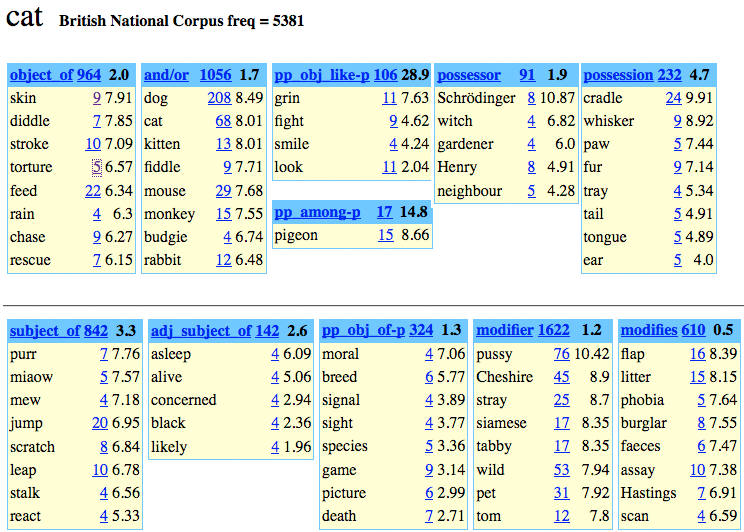
\includegraphics[width=10cm]{img/SE_cat}} ;
    \node[anchor=north east] at (10,0) {\tiny\light{\url{https://sketchengine.eu/}}} ;
  \end{tikzpicture}
\end{frame}

{\newcommand{\hg}[1]{\scriptsize\textpmhg{#1}}
\newcommand<>{\colA}[1]{\purered#2{#1}}
\newcommand<>{\colB}[1]{\puregreen#2{\textbf#2{#1}}}
\begin{frame}<beamer:1-4| handout:1-4>
  \frametitle{A thought experiment: deciphering hieroglyphs}
  % \framesubtitle{}

  \ungap[1]
  \begin{center}
    \setlength{\arrayrulewidth}{1pt}
    \begin{tabular}{@{\rule{0mm}{1.4em} }lr*{6}{|c}|}
      && \hg{get} & \hg{sij} & \hg{ius} & \hg{hir} & \hg{iit} & \hg{kil} \\
      \hline
      \tikz[remember picture, inner sep=0pt]{\node(knife){\colB<beamer:2| handout:2>{(knife)}}} & \colB<beamer:2| handout:2>{\hg{naif}} & \colB<beamer:2| handout:2>{51} & \colB<beamer:2| handout:2>{20} & \colB<beamer:2| handout:2>{84} &  \colB<beamer:2| handout:2>{0} &  \colB<beamer:2| handout:2>{3} &  \colB<beamer:2| handout:2>{0} \\
      \hline
      \tikz[remember picture, inner sep=0pt]{\node(cat){\colB<beamer:4| handout:4>{(cat)}}}   & \colB<beamer:4| handout:4>{\hg{ket}}  &  \colB<beamer:4| handout:4>{52} & \colB<beamer:4| handout:4>{58} &  \colB<beamer:4| handout:4>{4} &  \colB<beamer:4| handout:4>{4} &  \colB<beamer:4| handout:4>{6} & \colB<beamer:4| handout:4>{26} \\
      \hline
      \tikz[remember picture, inner sep=0pt]{\node(dog){\h{???}}} & \h{\hg{dog}} & \colA{115} & \colA{83} & \colA{10} & \colA{42} & \colA{33} & \colA{17} \\
      \hline
      (boat)  & \hg{beut} &  59 & 39 & 23 &  4 &  0 &  0 \\
      \hline
      (cup)   & \hg{kap}  &  98 & 14 &  6 &  2 &  1 &  0 \\
      \hline
      \tikz[remember picture, inner sep=0pt]{\node(pig){\colB<beamer:3| handout:3>{(pig)}}}  & \colB<beamer:3| handout:3>{\hg{pigij}} &  \colB<beamer:3| handout:3>{12} & \colB<beamer:3| handout:3>{17} &  \colB<beamer:3| handout:3>{3} &  \colB<beamer:3| handout:3>{2} &  \colB<beamer:3| handout:3>{9} & \colB<beamer:3| handout:3>{27} \\
      \hline
      (banana) & \hg{nana} & 11 &  2 &  2 &  0 & 18 &  0 \\
      \hline
    \end{tabular}
    
    \gap[2]\large
    \begin{tikzpicture}[remember picture, overlay]
      \draw<beamer:2| handout:2>[<->,puregreen,very thick] (dog.west) to[out=160, in=200] (knife.west) ;
      \draw<beamer:3| handout:3>[<->,puregreen,very thick] (dog.west) to[out=210, in=150] (pig.west) ;
      \draw<beamer:4| handout:4>[<->,puregreen,very thick] (dog.west) to[out=150, in=210] (cat.west) ;
    \end{tikzpicture}
    \only<beamer:2| handout:2>{%
      sim(\colA{\hg{dog}}, \colB{\hg{naif}}) = 0.770 }%
    \only<beamer:3| handout:3>{%
      sim(\colA{\hg{dog}}, \colB{\hg{pigij}}) = 0.939 }%
    \only<beamer:4| handout:4>{%
      sim(\colA{\hg{dog}}, \colB{\hg{ket}}) = 0.961 }%
  \end{center}

  \addnote{Similarity scores are cosine similarities on sparse log-scaled frequencies ($\log (f+1)$).}%
\end{frame}

\begin{frame}
  \frametitle{English as seen by the computer \ldots}
  % \framesubtitle{}

  \begin{center}
    \ungap[1]
    \setlength{\arrayrulewidth}{1pt}
    \begin{tabular}{@{\rule{0mm}{1.4em} }l@{ }r*{6}{|c}|}
      && get & see & use & hear & eat & kill \\[-0.4em]
      && \hg{get} & \hg{sij} & \hg{ius} & \hg{hir} & \hg{iit} & \hg{kil} \\
      \hline
      knife & \hg{naif} &  51 & 20 & 84 &  0 &  3 &  0 \\
      \hline
      cat   & \hg{ket}  &  52 & 58 &  4 &  4 &  6 & 26 \\
      \hline
      \h{dog} & \h{\hg{dog}} & \colA{115} & \colA{83} & \colA{10} & \colA{42} & \colA{33} & \colA{17} \\
      \hline
      boat  & \hg{beut} &  59 & 39 & 23 &  4 &  0 &  0 \\
      \hline
      cup   & \hg{kap}  &  98 & 14 &  6 &  2 &  1 &  0 \\
      \hline
      pig  & \hg{pigij} &  12 & 17 &  3 &  2 &  9 & 27 \\
      \hline
      banana & \hg{nana} & 11 &  2 &  2 &  0 & 18 &  0 \\
      \hline
    \end{tabular}
  \end{center}
  \hfill\light{\footnotesize verb-object counts from British National Corpus}
\end{frame}
}

\begin{frame}
  \frametitle{Geometric interpretation}
  % \framesubtitle{}

  \begin{columns}[T]
    \begin{column}{40mm}
      \begin{itemize}
      \item row vector \primary{$\vx_{\text{dog}}$} describes usage of word \emph{dog} in the corpus
      \item can be seen as coordinates of point in $n$-dimensional Euclidean space
       \end{itemize}
    \end{column}
    \begin{column}{75mm}      
      \gap[2]
      \begin{small}
        \setlength{\arrayrulewidth}{1pt}
        \begin{tabular}{r*{6}{|c}|}
          & get & see & use & hear & eat & kill \\
          \hline
          knife &  51 & 20 & 84 &  0 &  3 &  0 \\
          \hline
          cat  &  52 & 58 &  4 &  4 &  6 & 26 \\
          \hline
          \h{dog} & \primary{115} & \primary{83} & \primary{10} & \primary{42} & \primary{33} & \primary{17} \\
          \hline
          boat &  59 & 39 & 23 &  4 &  0 &  0 \\
          \hline
          cup  &  98 & 14 &  6 &  2 &  1 &  0 \\
          \hline
          pig  &  12 & 17 &  3 &  2 &  9 & 27 \\
          \hline
          banana & 11 &  2 &  2 &  0 & 18 &  0 \\
          \hline
        \end{tabular}
      \end{small}

      \begin{center}
        \h{co-occurrence matrix} $\mathbf{M}$
      \end{center}
    \end{column}
  \end{columns}
\end{frame}

\begin{frame}
  \frametitle{Geometric interpretation}
  % \framesubtitle{}

  \begin{columns}[T]
    \begin{column}{40mm}
      \begin{itemize}
      \item row vector \primary{$\vx_{\text{dog}}$} describes usage of word \emph{dog} in the corpus
      \item can be seen as coordinates of point in $n$-dimensional Euclidean space
      \item illustrated for two dimensions:\\ \emph{get} and \emph{use}
      \item \primary{$\vx_{\text{dog}} = (115,10)$}
      \end{itemize}
    \end{column}
    \begin{column}{75mm}      
      \ungap[1]
      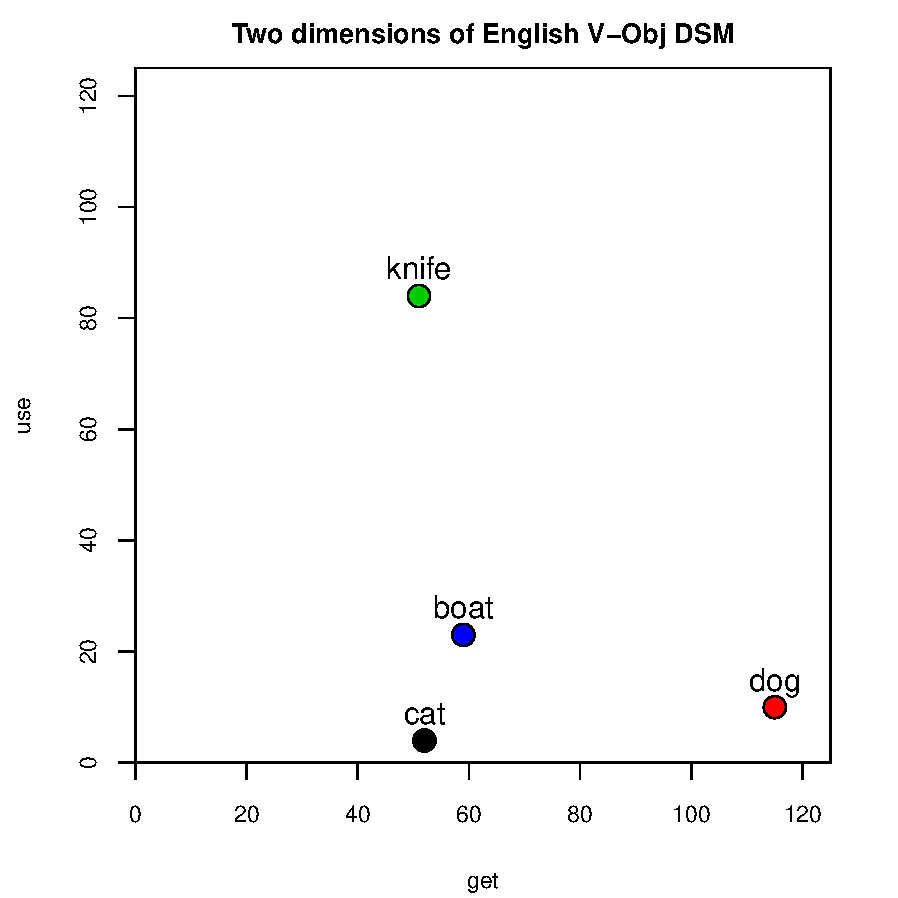
\includegraphics[width=75mm]{img/hieroglyph_2d_1}
    \end{column}
  \end{columns}
\end{frame}

\begin{frame}
  \frametitle{Geometric interpretation}
  % \framesubtitle{}

  \begin{columns}[T]
    \begin{column}{40mm}
      \begin{itemize}
      \item similarity = spatial proximity (Euclidean dist.)
      \item location depends on frequency of noun ($f_{\text{dog}} \approx 2.7\cdot f_{\text{cat}}$)
      \end{itemize}
    \end{column}
    \begin{column}{75mm}      
      \ungap[1]
      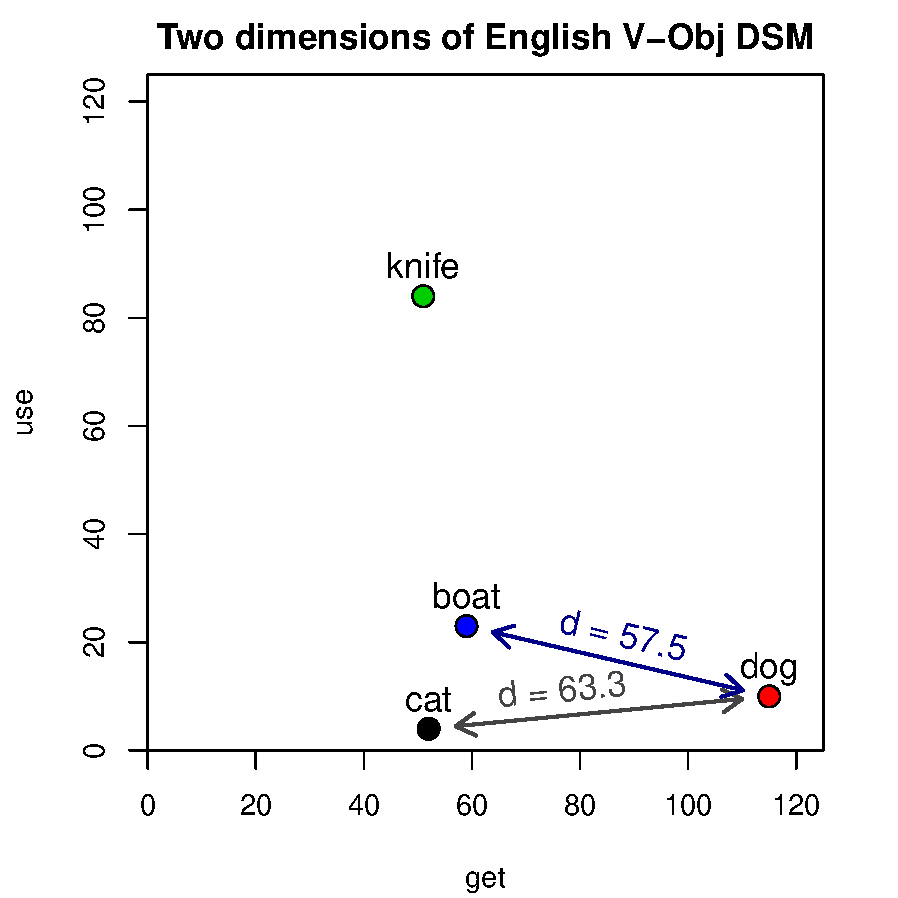
\includegraphics[width=75mm]{img/hieroglyph_2d_2}
    \end{column}
  \end{columns}
\end{frame}

\begin{frame}<beamer:1| handout:0>
  \frametitle{Geometric interpretation}
  % \framesubtitle{}

  \begin{columns}[T]
    \begin{column}{40mm}
      \begin{itemize}
      \item vector can also be understood as arrow from origin
      \item direction more important than location
      \end{itemize}
    \end{column}
    \begin{column}{75mm}      
      \ungap[1]
      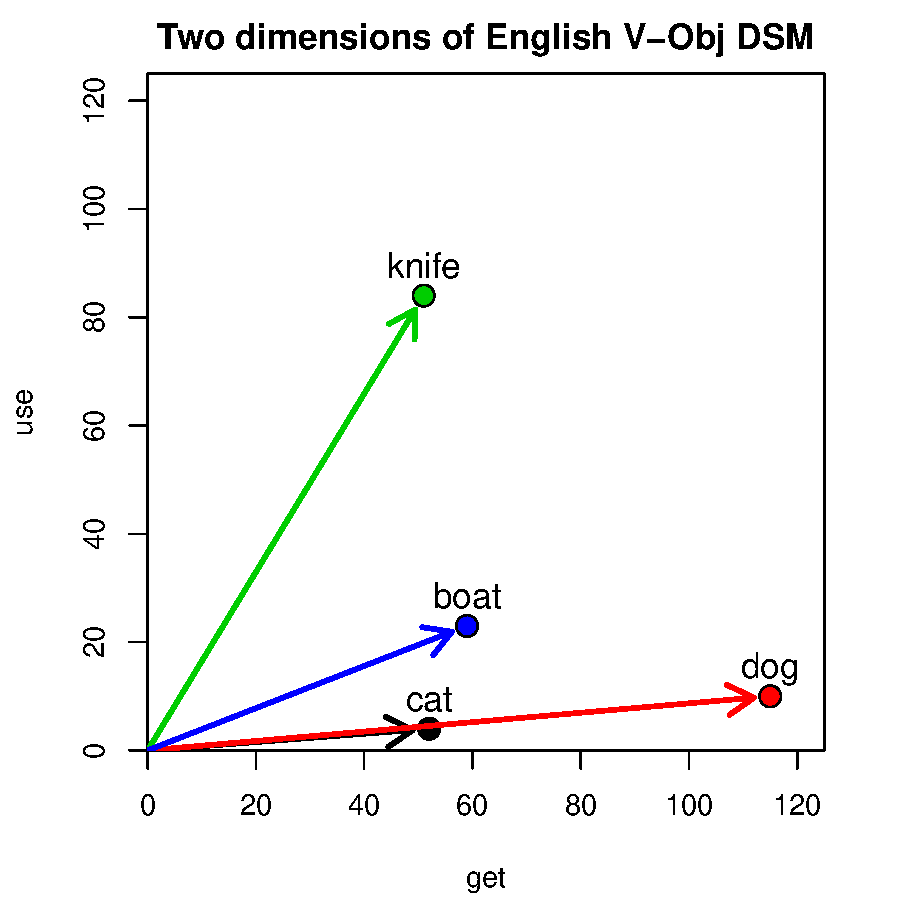
\includegraphics[width=75mm]{img/hieroglyph_2d_3}
    \end{column}
  \end{columns}
\end{frame}

\begin{frame}
  \frametitle{Geometric interpretation}
  % \framesubtitle{}

  \begin{columns}[T]
    \begin{column}{40mm}
      \begin{itemize}
      \item vector can also be understood as arrow from origin
      \item direction more important than location
      \item<beamer:1-| handout:1-> use angle $\alpha$ as distance measure
      \item<beamer:2-| handout:2-> or normalise length $\norm{\vx_{\text{dog}}}$ of arrow
      \end{itemize}
    \end{column}
    \begin{column}{75mm}
      \ungap[1]
      \only<beamer:1| handout:1>{%
        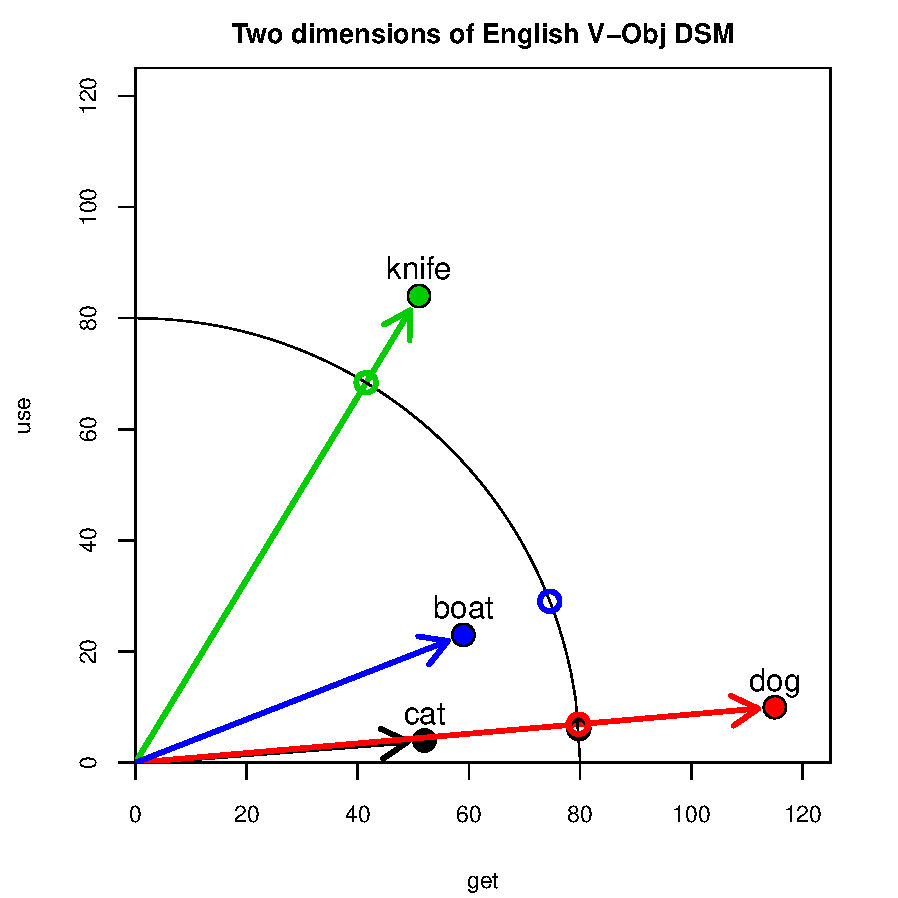
\includegraphics[width=75mm]{img/hieroglyph_2d_4}}%
      \only<beamer:2| handout:2>{%
        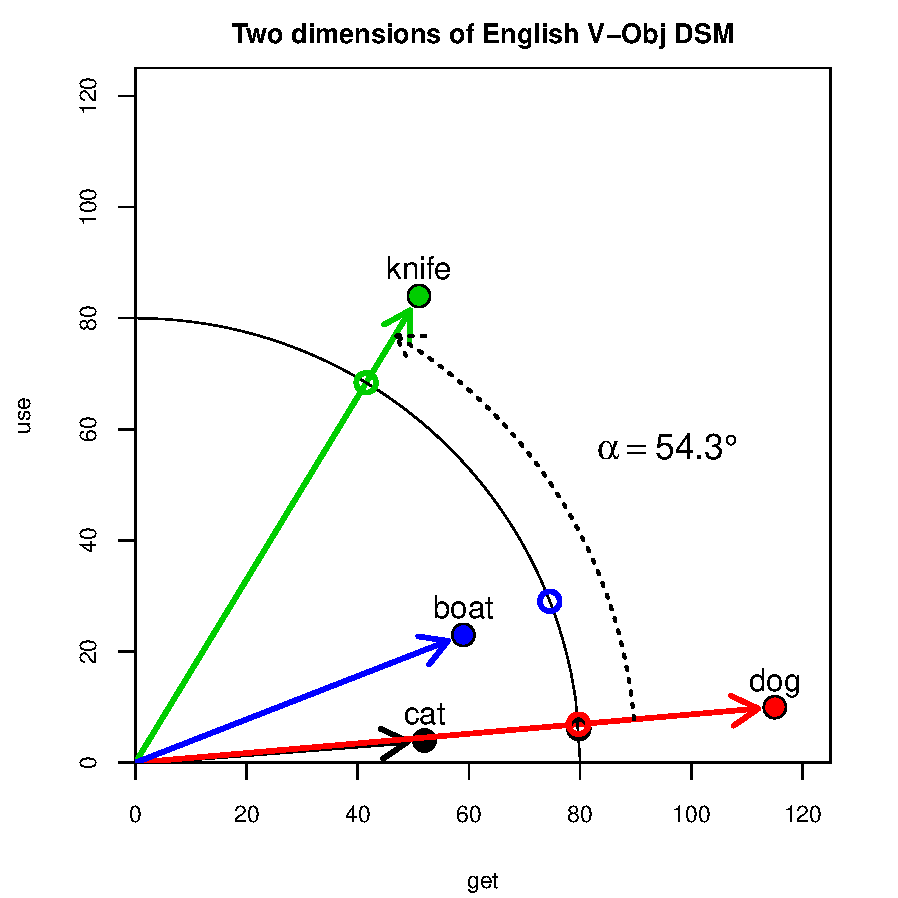
\includegraphics[width=75mm]{img/hieroglyph_2d_5}}%
    \end{column}
  \end{columns}
\end{frame}

%%%%%%%%%%%%%%%%%%%%%%%%%%%%%%%%%%%%%%%%%%
\subsection{Distributional semantic models}

\begin{frame}
  \frametitle{General definition of DSMs}
  % \framesubtitle{}

  \ungap
  \begin{block}{}
    A \h{distributional semantic model} (DSM) is a scaled and/or
    transformed co-occurrence matrix $\mathbf{M}$, such that each row $\vx$
    represents the distribution of a target term across contexts.
  \end{block}

  \begin{center}
    \begin{small}
      \setlength{\arrayrulewidth}{1pt}
      \begin{tabular}{r*{6}{|c}|}
        & get & see & use & hear & eat & kill \\
        \hline
        knife &  0.027 & -0.024 &  0.206 & -0.022 & -0.044 & -0.042 \\
        \hline
        cat   &  0.031 &  0.143 & -0.243 & -0.015 & -0.009 &  0.131 \\
        \hline
        \primary{dog}   & \primary{-0.026} &  \primary{0.021} & \primary{-0.212} &  \primary{0.064} &  \primary{0.013} &  \primary{0.014} \\
        \hline
        boat  & -0.022 &  0.009 & -0.044 & -0.040 & -0.074 & -0.042 \\
        \hline
        cup   & -0.014 & -0.173 & -0.249 & -0.099 & -0.119 & -0.042 \\
        \hline
        pig   & -0.069 &  0.094 & -0.158 &  0.000 &  0.094 &  0.265 \\
        \hline
        banana&  0.047 & -0.139 & -0.104 & -0.022 &  0.267 & -0.042 \\
        \hline
      \end{tabular}
    \end{small}
  \end{center}

  \hh{Term} = word, lemma, phrase, morpheme, word pair, \ldots
\end{frame}

\begin{frame}
  \frametitle{Nearest neighbours}
  \framesubtitle{DSM based on verb-object relations from BNC, reduced to 100 dim.\ with SVD}
  % \framesubtitle{}

  Neighbours of \h{trousers} (cosine angle):
  \begin{itemize}\item[\hand]
    shirt (18.5), blouse (21.9), scarf (23.4), jeans (24.7), skirt (25.9),
    sock (26.2), shorts (26.3), jacket (27.8), glove (28.1), coat (28.8),
    cloak (28.9), hat (29.1), tunic (29.3), overcoat (29.4), pants (29.8),
    helmet (30.4), apron (30.5), robe (30.6), mask (30.8), tracksuit (31.0),
    jersey (31.6), shawl (31.6), \ldots
  \end{itemize}

  \gap\pause
  Neighbours of \h{rage} (cosine angle):
  \begin{itemize}\item[\hand]
    anger (28.5), fury (32.5), sadness (37.0), disgust (37.4), emotion (39.0),
    jealousy (40.0), grief (40.4), irritation (40.7), revulsion (40.7), scorn
    (40.7), panic (40.8), bitterness (41.6), resentment (41.8), indignation
    (41.9), excitement (42.0), hatred (42.5), envy (42.8), disappointment
    (42.9), \ldots 
  \end{itemize}
  \addnote{Neighbours and neighbourhood plots from BNC verb-object DSM, reduced to 100 dimensions by SVD.}%
\end{frame}

\begin{frame}[c]
  \frametitle{Nearest neighbours with similarity graph}
  % \framesubtitle{}

  \ungap[1]
  \begin{center}
    \only<beamer:0| handout:1>{%
      \begin{tabular}{@{}cc@{}}
        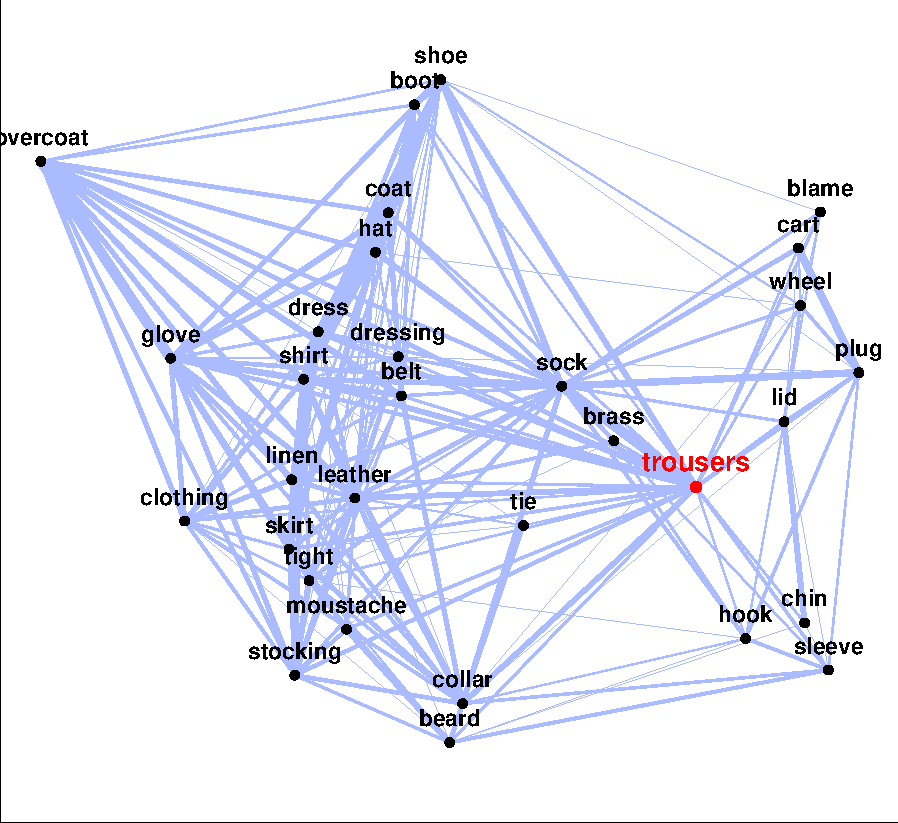
\includegraphics[width=55mm]{img/neighbourhood_trousers} 
        & 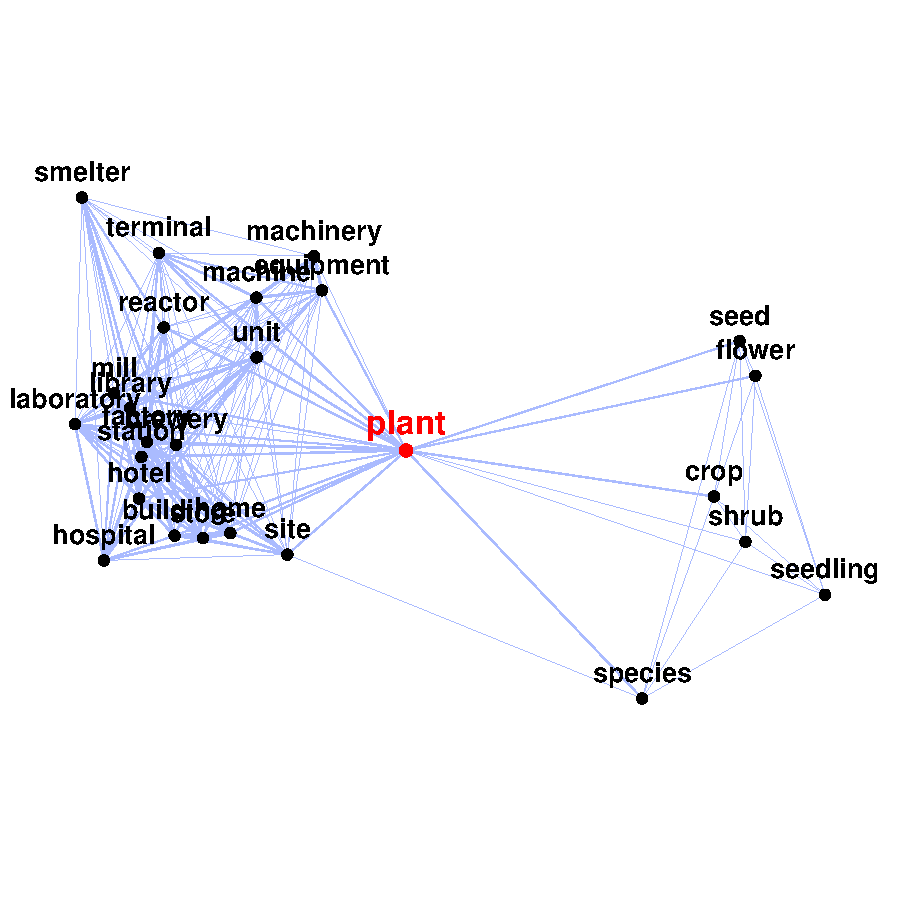
\includegraphics[width=55mm]{img/neighbourhood_plant}
      \end{tabular}}%
    \only<beamer:1| handout:0>{%
       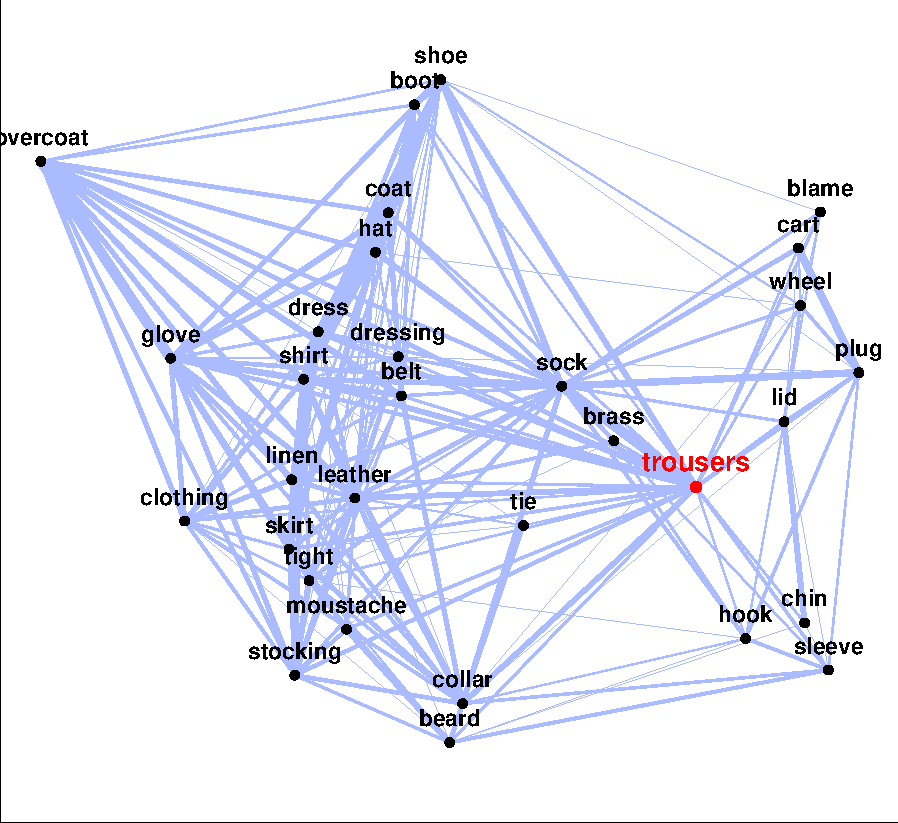
\includegraphics[width=75mm]{img/neighbourhood_trousers}}%
    \only<beamer:2| handout:0>{%
      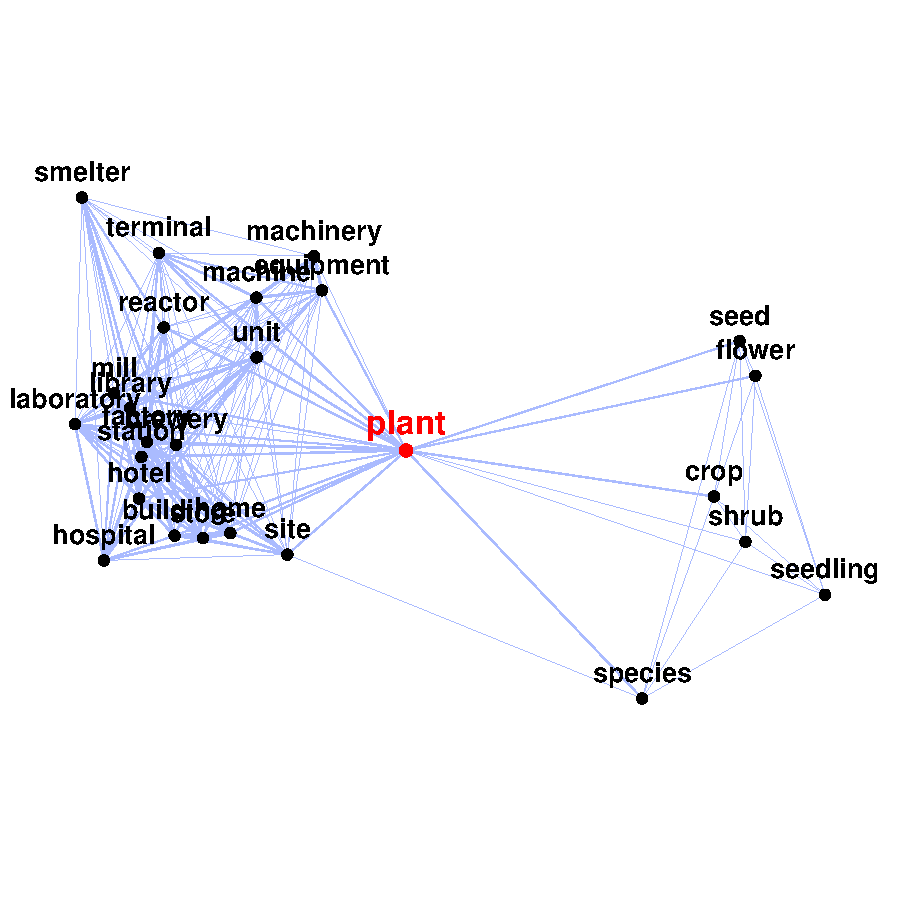
\includegraphics[width=90mm, trim=0 50 0 50, clip]{img/neighbourhood_plant}}%
  \end{center}
\end{frame}

\begin{frame}[c]
  \frametitle{Semantic maps}
  % \framesubtitle{}

  \ungap[1]
  \begin{center}
    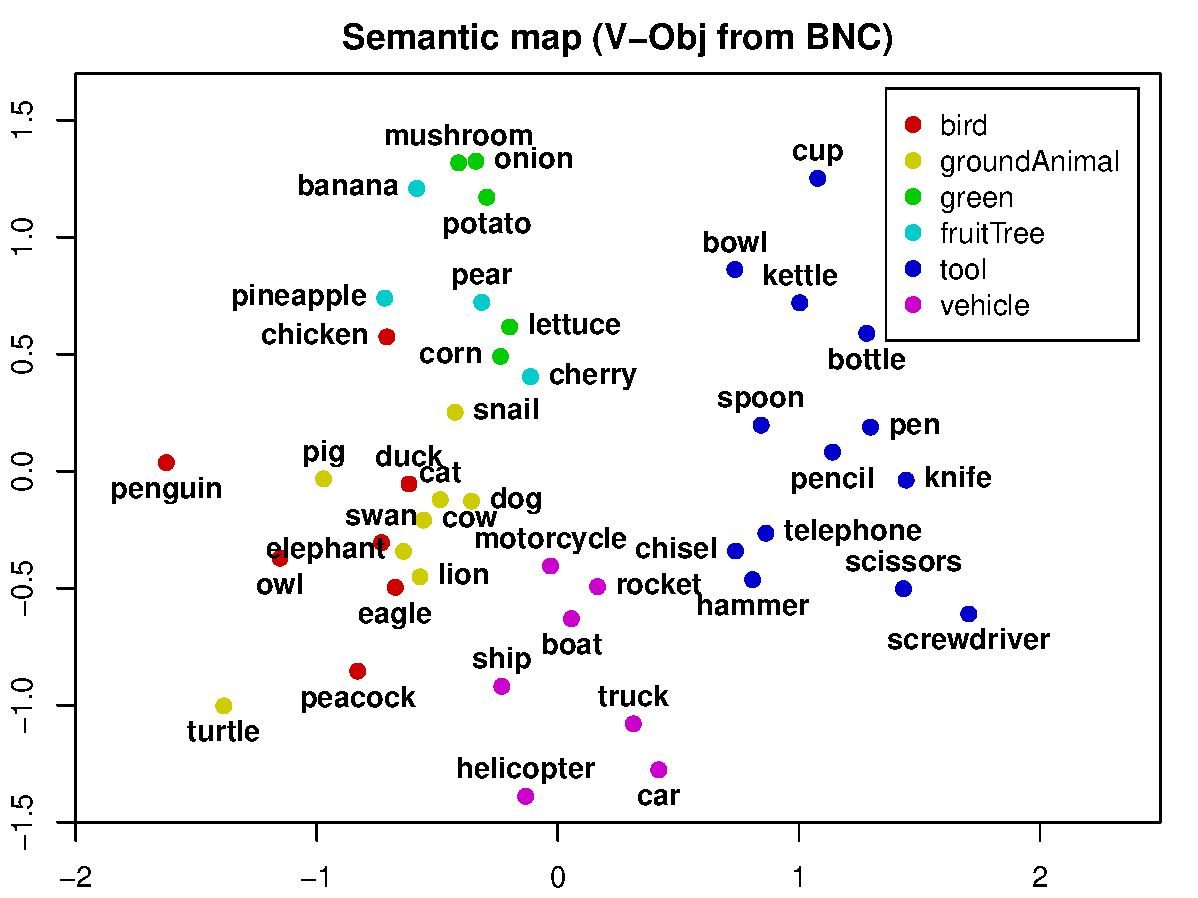
\includegraphics[width=100mm]{img/vobj_semantic_map}
  \end{center}
  \addnote{Roughly horizontal axis separates natural objects (left) from artifacts (right), or animate vs. inanimate There is a clear boundary between the two groups}%
  \addnote{Orthogonal axis separates moving things (bottom) from motionless ones (top).}%
\end{frame}

\begin{frame}[c]
  \frametitle{Clustering}
  % \framesubtitle{}

  \ungap[1]
  \begin{center}
    \only<beamer:1| handout:1>{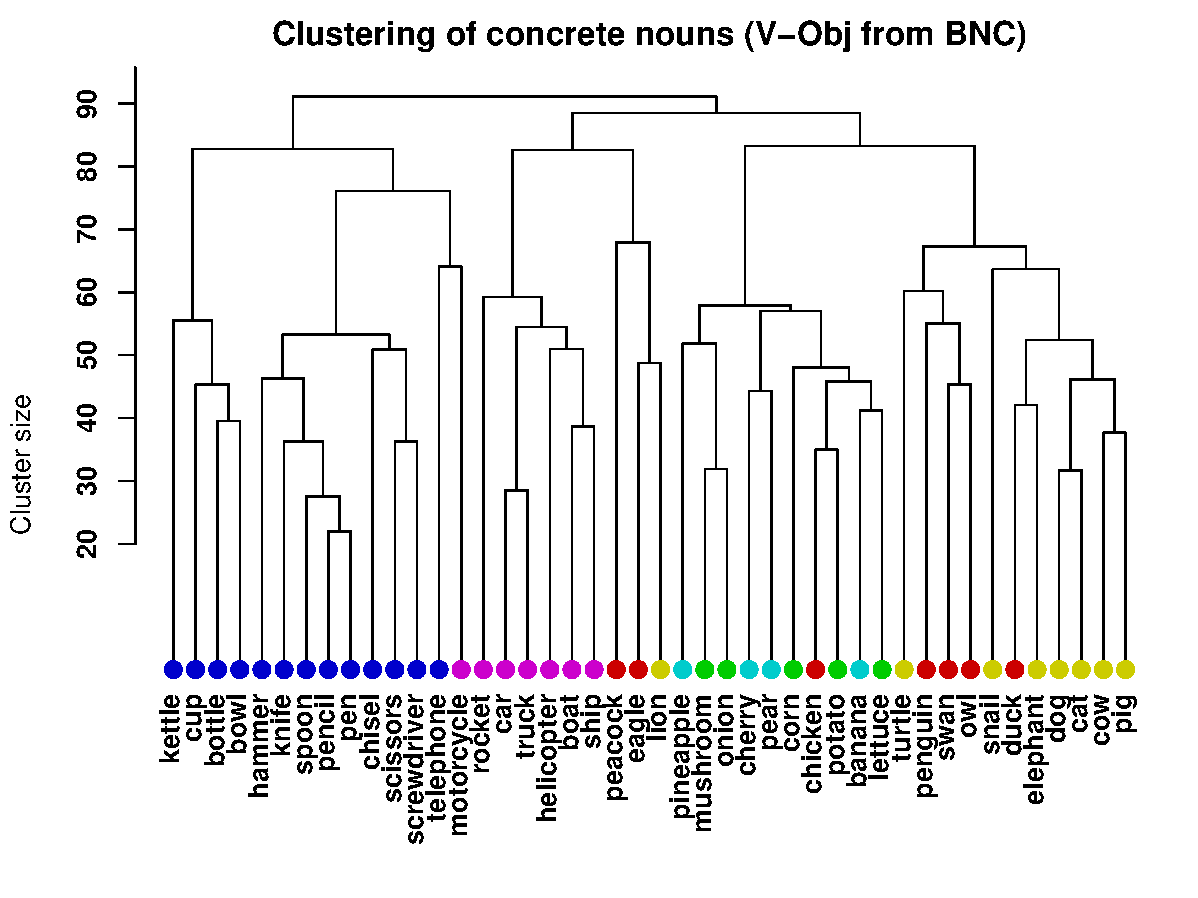
\includegraphics[width=100mm]{img/vobj_clustering}}%
    \only<beamer:2| handout:0>{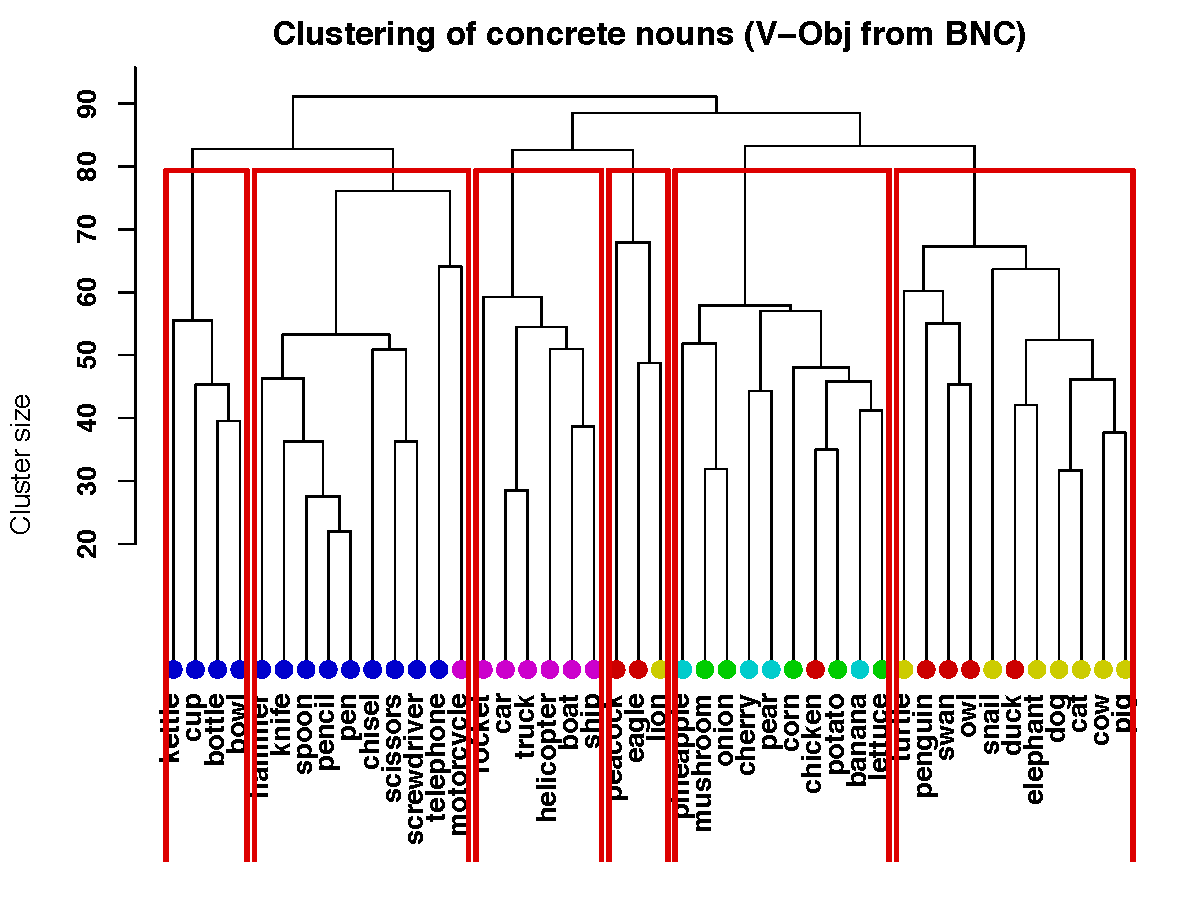
\includegraphics[width=100mm]{img/vobj_clustering_6}}%
  \end{center}
\end{frame}

\begin{frame}[c]
  \frametitle{Latent ``meaning'' dimensions}
  % \framesubtitle{}

  \ungap[1]
  \begin{center}
    \only<beamer:1| handout:0>{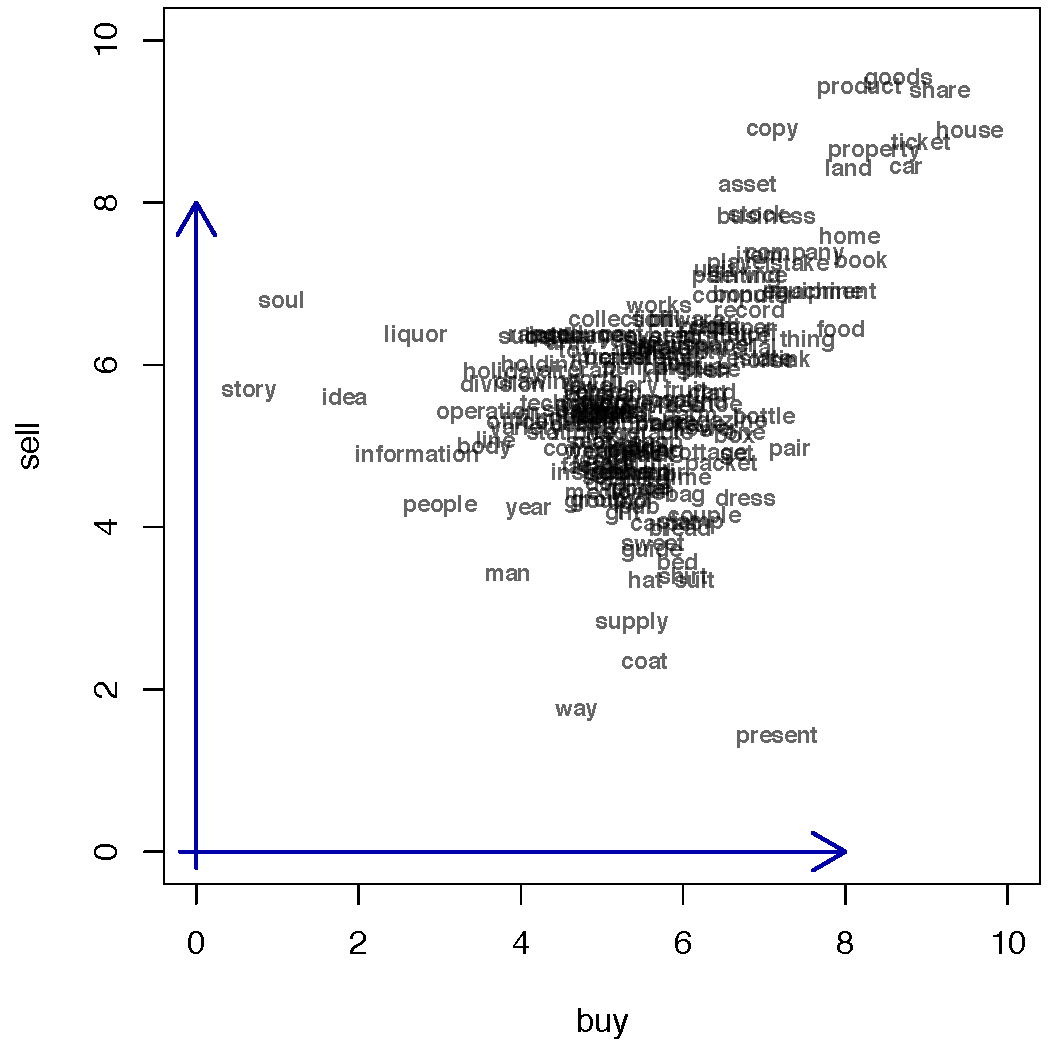
\includegraphics[width=8cm]{img/buy_sell_labels_only}}
    \only<beamer:2| handout:1>{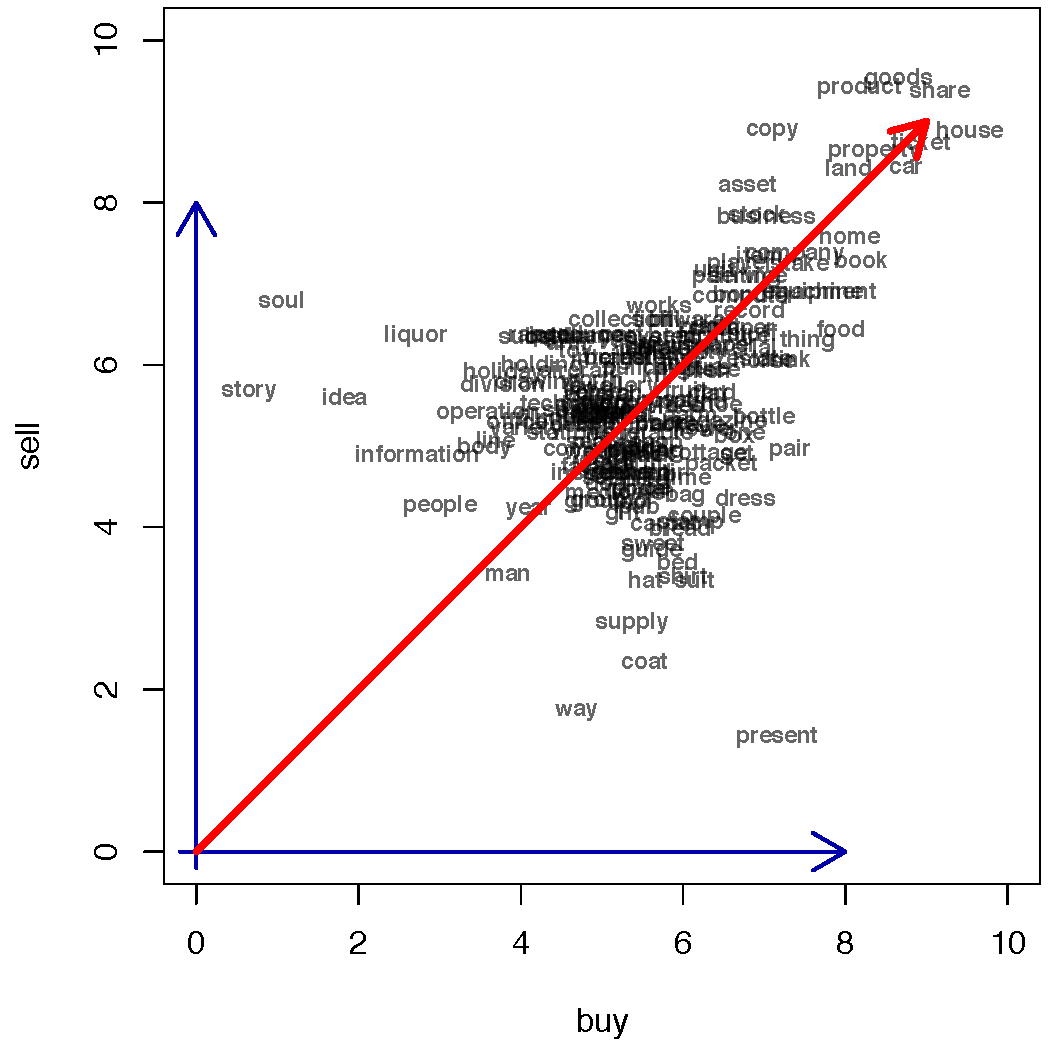
\includegraphics[width=8cm]{img/buy_sell_labels_latent}}
  \end{center}
\end{frame}

\begin{frame}
  \frametitle{DSM vectors as word embeddings}

  \begin{columns}[T]
    \begin{column}{60mm}
      DSM vector as sub-symbolic meaning representation
      \begin{itemize}
      \item feature vector for machine learning algorithm
      \item input for neural network
      \item such \primary{distributed} representations are known as \hh{embeddings}
      \itemhand embeddings $\not\Rightarrow$ distributional
      \end{itemize}

      \gap[1]
      \onslide<2->
      Computation in semantic space
      \begin{itemize}
      \item find meaningful subdimensions in DSM space (\so correlation)
      \item linear operations on vectors
      \end{itemize}
    \end{column}
    \begin{column}{50mm}
      \onslide<1->\ungap[2]
      \begin{center}
        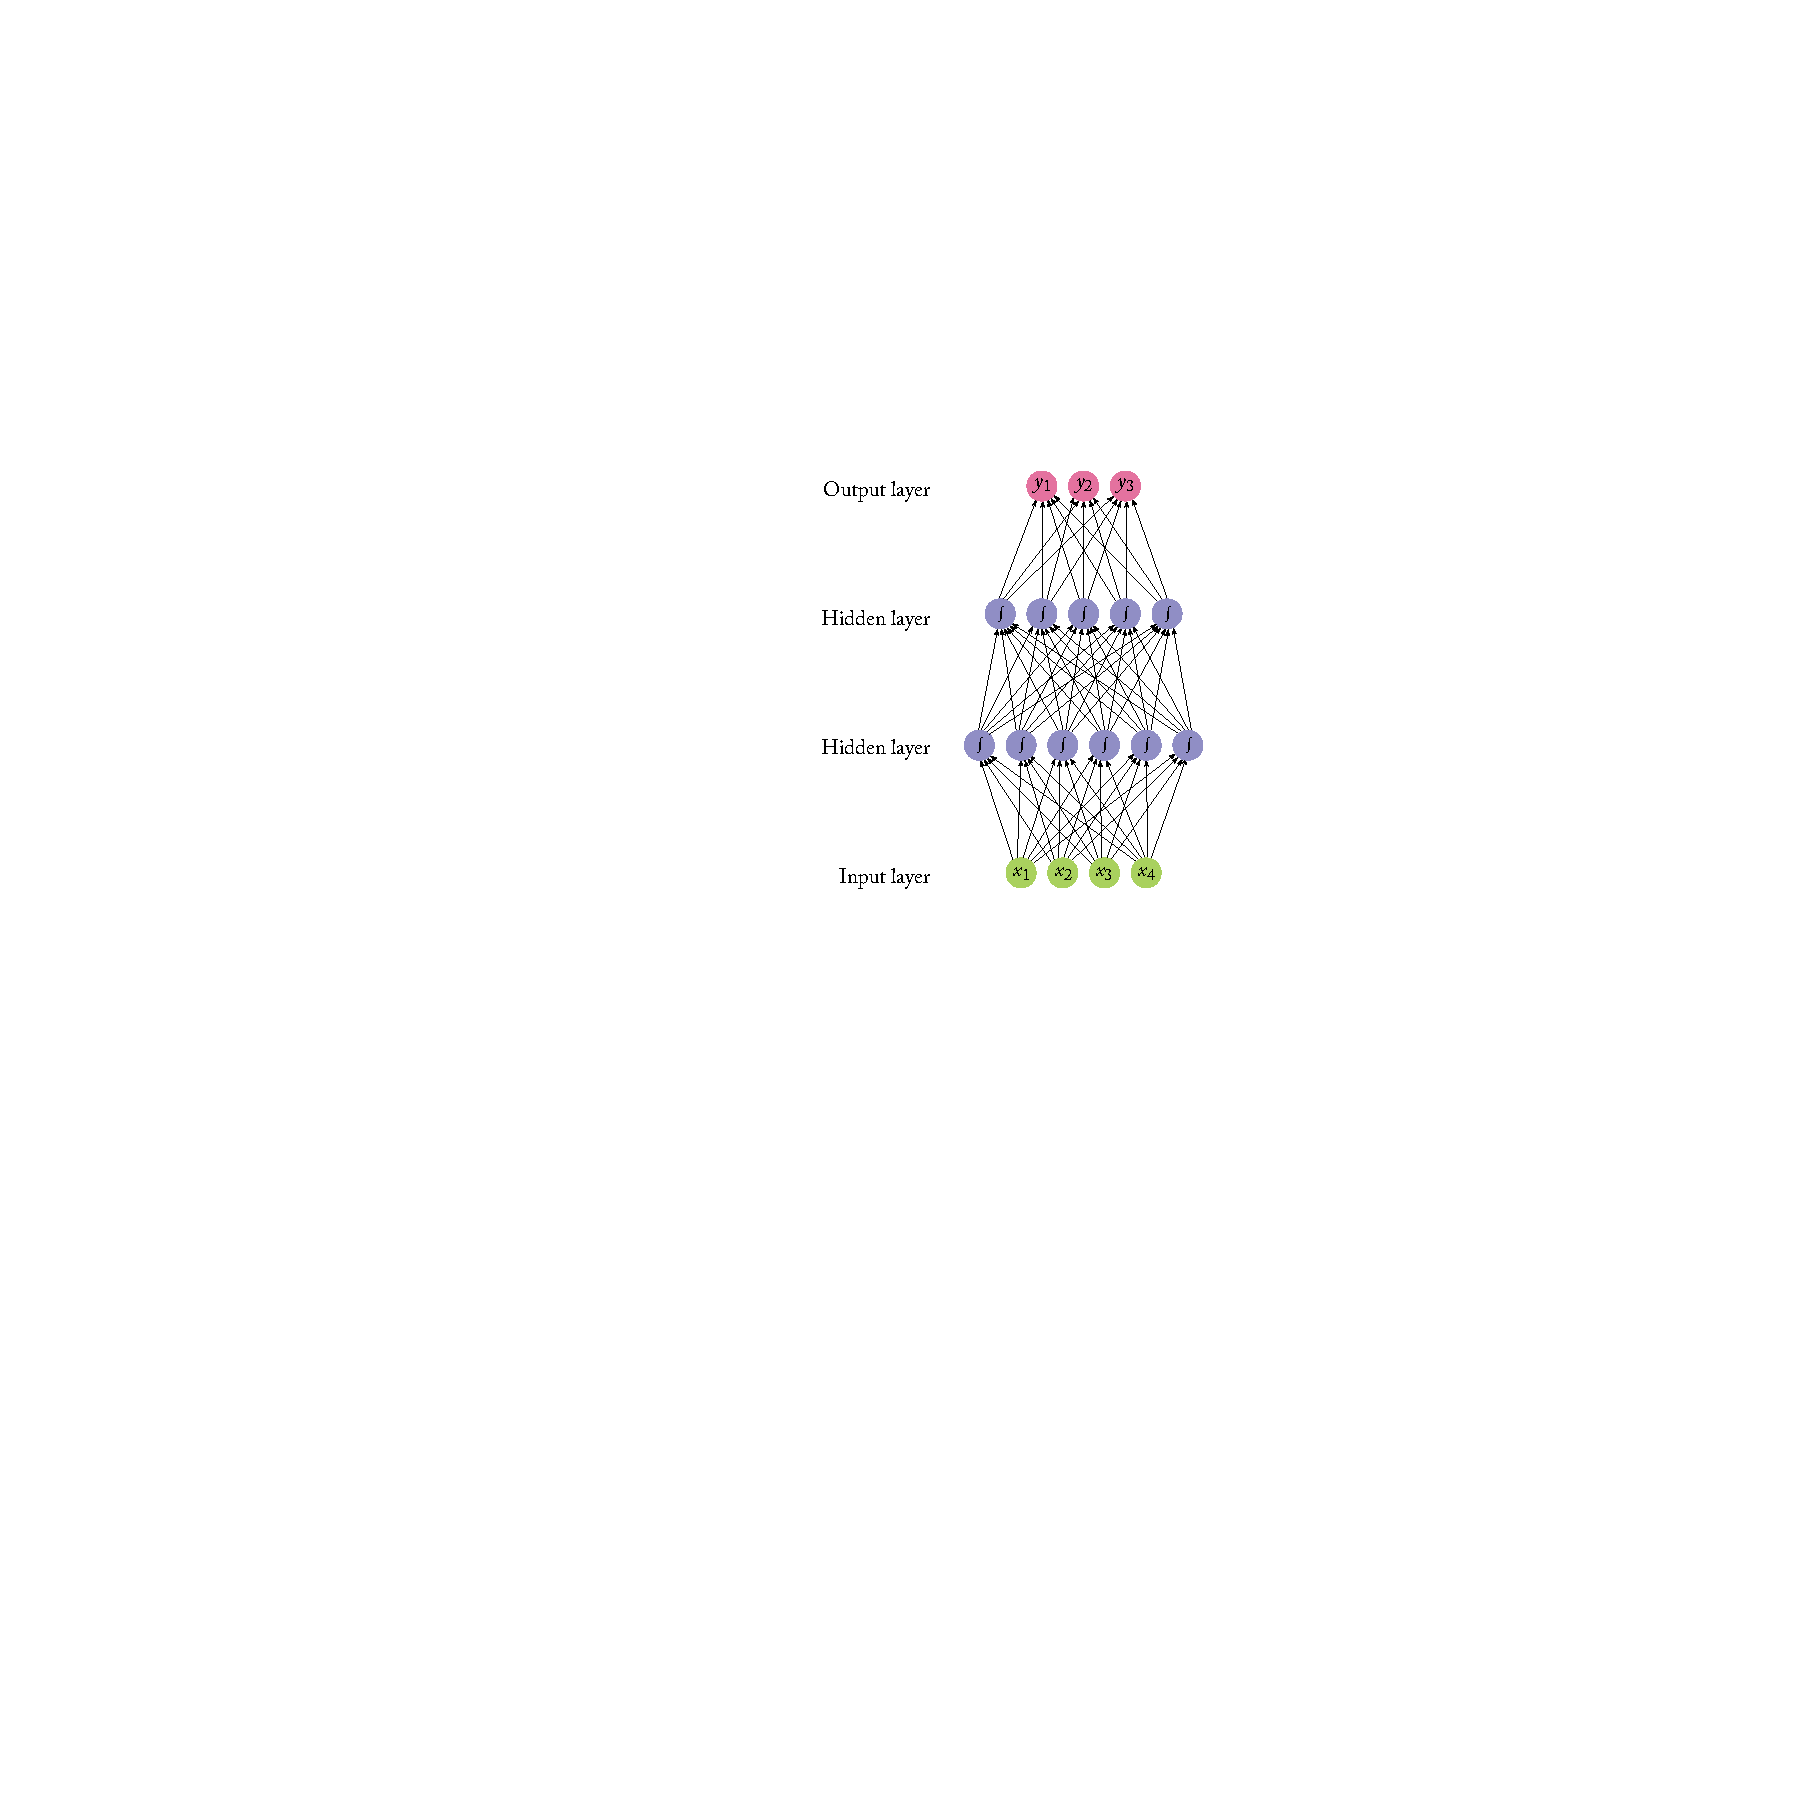
\includegraphics[width=35mm]{img/Goldberg2017_Fig4_2}
      \end{center}
      \ungap[1]
      {\tiny \hfill\citep[Fig.~4.2]{Goldberg:17}}
      \onslide<2->
      \begin{center}
        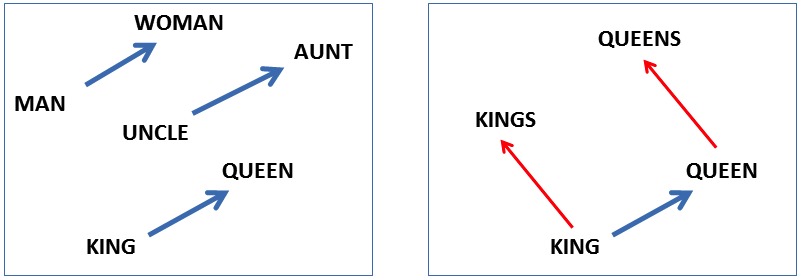
\includegraphics[width=30mm, trim={14cm 0 0 0}, clip]{img/MikolovYihZweig2013_Fig2}
      \end{center}
      \ungap[1]
      {\tiny \hfill\citep[Fig.~2]{Mikolov:Yih:Zweig:13}}
    \end{column}
  \end{columns}
\end{frame}

\begin{frame}
  \frametitle{DSM vectors as context representation}

  \begin{columns}[T]
    \begin{column}{60mm}
      \h{Context vectors} for word tokens \citep{Schuetze:98} 
      \begin{itemize}
      \item \hh{bag-of-words} approach:
        centroid of all context words in the sentence
      \item application to WSD
      \end{itemize}
    \end{column}
    \begin{column}{60mm}
      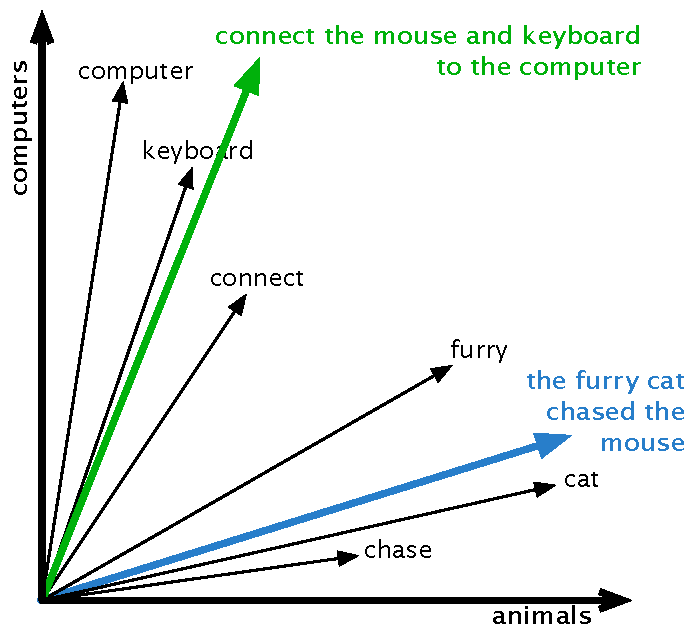
\includegraphics[width=60mm]{img/illustration_context_vectors_mouse}
    \end{column}
  \end{columns}
\end{frame}


%%%%%%%%%%%%%%%%%%%%%%%%%%%%%%%%%%%%%%%%%%
\subsection{DSMs and semantic similarity}

\begin{frame}[c]
\frametitle{Inverse distributional semantics}
\framesubtitle{Which word occurs in similar contexts as the ones displayed in this graph?}
\centering
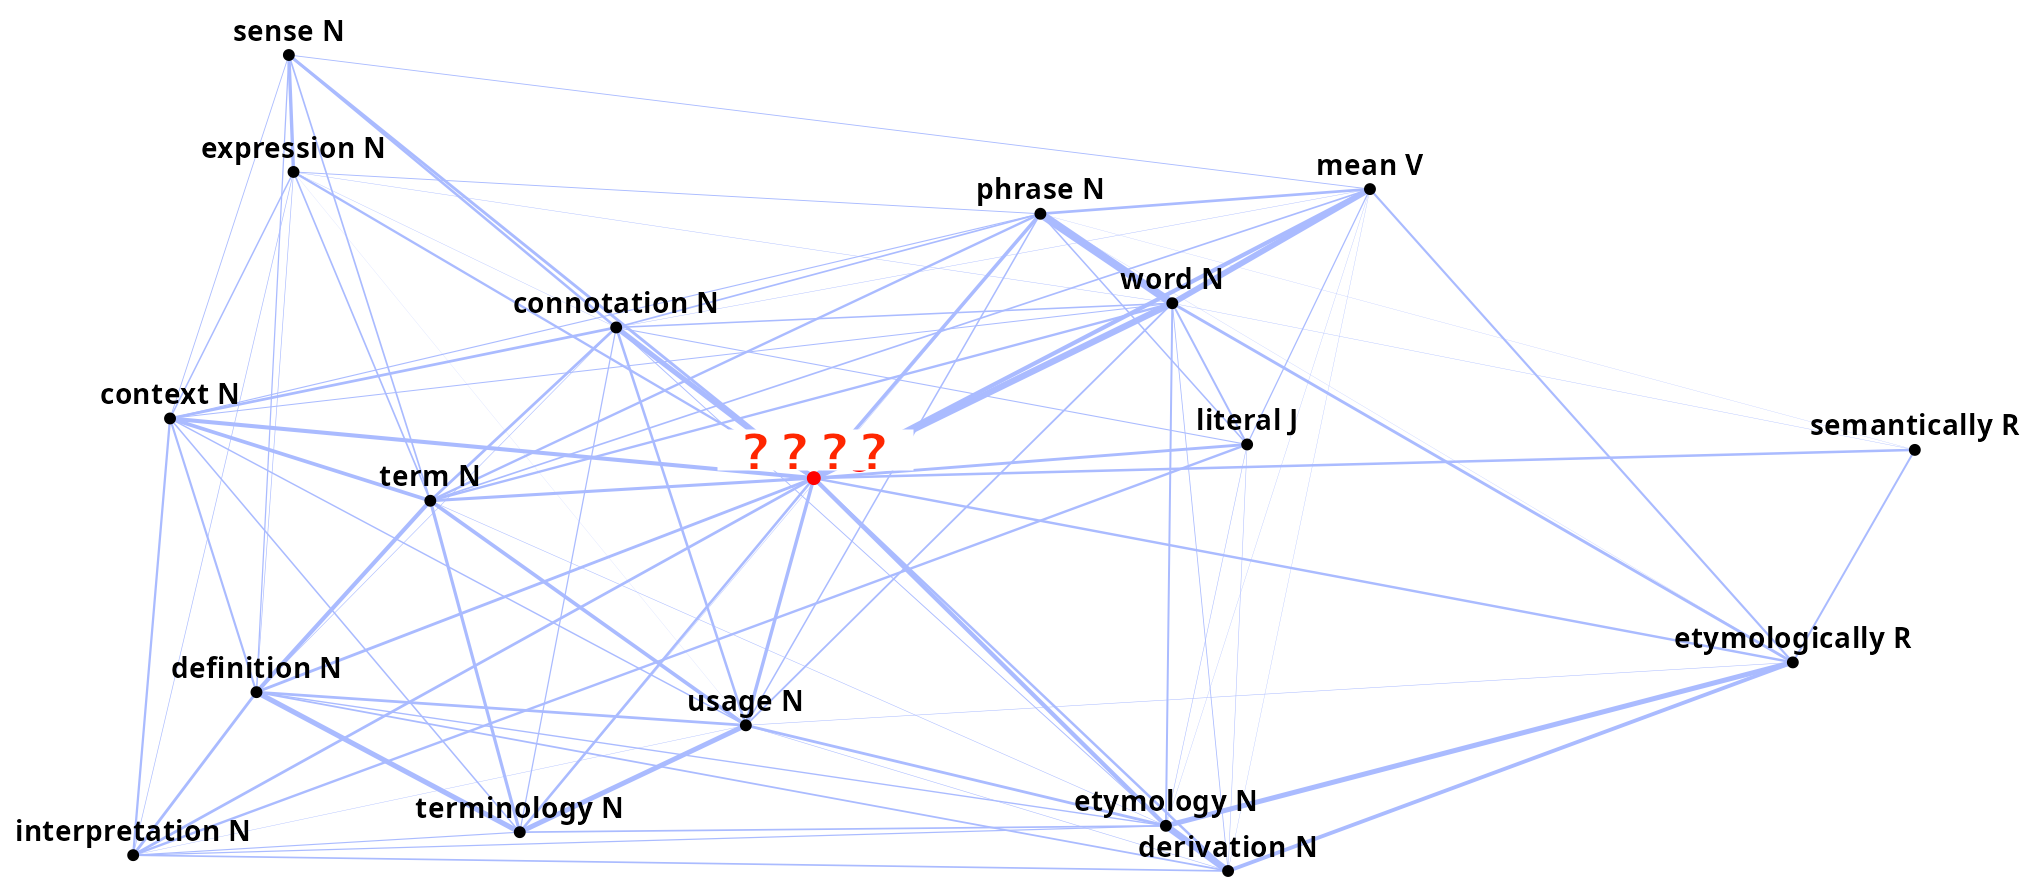
\includegraphics[width=\textwidth]{img/masked_neighbours_meaning}

\raggedleft\gap
\ldots{} look at the neighbours:\\
is there one notion of similarity that explains all of them?
\end{frame}

\begin{frame}
  \frametitle{Distributional similarity as semantic similarity}

  \begin{itemize}
  \item DSM similarity as a \primary{quantitative notion} \citep{Harris:54}
    \begin{itemize}
    \item if $\va$ is closer to $\vb$ than to $\Vector{c}$ in the distributional
      vector space, then $a$ is more semantically similar to $b$ than to $c$
    \end{itemize}
    \bigskip
  \item DSM similarity as a  \primary{graded notion}, differently from \secondary{categorical} nature of most theoretical accounts
     \bigskip 
  \item DSM similarity as the empirical correlate of a \primary{heterogeneous set of phenomena}\\
  	\hfill ... which we may want to tease apart! 
\bigskip
  \item DSM similarity is \primary{symmetric} -- cognition is not \\
  	\hfill ... can we fix this? 	
    \end{itemize}
\end{frame}


\begin{frame}
  \frametitle{Characterising DSM similarity}
  \begin{itemize}
   \item DSMs are often thought to represent \primary{taxonomic} similarity
   \begin{itemize}
    \item words that tend to occur in the same contexts
    \item[]
    \end{itemize}
  \item Words that share many contexts share many properties (attributes) and are thus 
    \secondary{taxonomically/ontologically similar}
    \begin{itemize}
    \item synonyms (\emph{rhino/rhinoceros})
    \item antonyms and values on a scale (\emph{good/bad})
    \item co-hyponyms (\emph{rock/jazz})
    \item hyper- and hyponyms (\emph{rock/basalt})
    \item[]
    \end{itemize}
  \item Taxonomic similarity is seen as the \primary{fundamental semantic relation} organising the vocabulary of a language, allowing categorisation, generalisation and inheritance...
  \end{itemize}
\end{frame}


\begin{frame}
  \frametitle{Is distributional similarity \textit{just} taxonomic?}

  \ungap[.5]
  Nearest DSM neighbors have different types of \primary{semantic relations}.

  \ungap[.5]\footnotesize
  \begin{columns}[t]
    \column{5cm}
    \begin{block}{\emph{car} {\small (BNC, L2/R2 span)}}
      \begin{itemize}
      \item van {\color{counterpoint} co-hyponym}
      \item vehicle {\color{counterpoint} hyperonym}
      \item truck {\color{counterpoint} co-hyponym}
      \item motorcycle {\color{counterpoint} co-hyponym}
      \item driver {\color{counterpoint} related entity}
      \item motor {\color{counterpoint} part}
      \item lorry {\color{counterpoint} co-hyponym}
      \item motorist {\color{counterpoint} related entity}
      \item cavalier {\color{counterpoint} hyponym}
      \item bike {\color{counterpoint} co-hyponym}
      \end{itemize}
    \end{block}
    \column{5cm}
    \begin{block} {\emph{car} {\small (BNC, L30/R30 span)}}
      \begin{itemize}
      \item drive {\color{counterpoint} function}
      \item park {\color{counterpoint} typical action}
      \item bonnet {\color{counterpoint} part}
      \item windscreen {\color{counterpoint} part}
      \item hatchback {\color{counterpoint} part}
      \item headlight {\color{counterpoint} part}
      \item jaguar {\color{counterpoint} hyponym}
      \item garage {\color{counterpoint} location}
      \item cavalier {\color{counterpoint} hyponym}
      \item tyre {\color{counterpoint} part}
      \end{itemize}
    \end{block}
  \end{columns}

  \hfill\light{\tiny \url{http://clic.cimec.unitn.it/infomap-query/}}
\end{frame}

\begin{frame}
  \frametitle{Is distributional similarity \textit{just} taxonomic?}
  \framesubtitle{Manual annotation: what are the properties of \primary{\textit{car}}? Humans vs DSM}

  \ungap[1]
  \begin{columns}[c]
    \begin{column}{6cm}
      \hspace*{-1em}%
      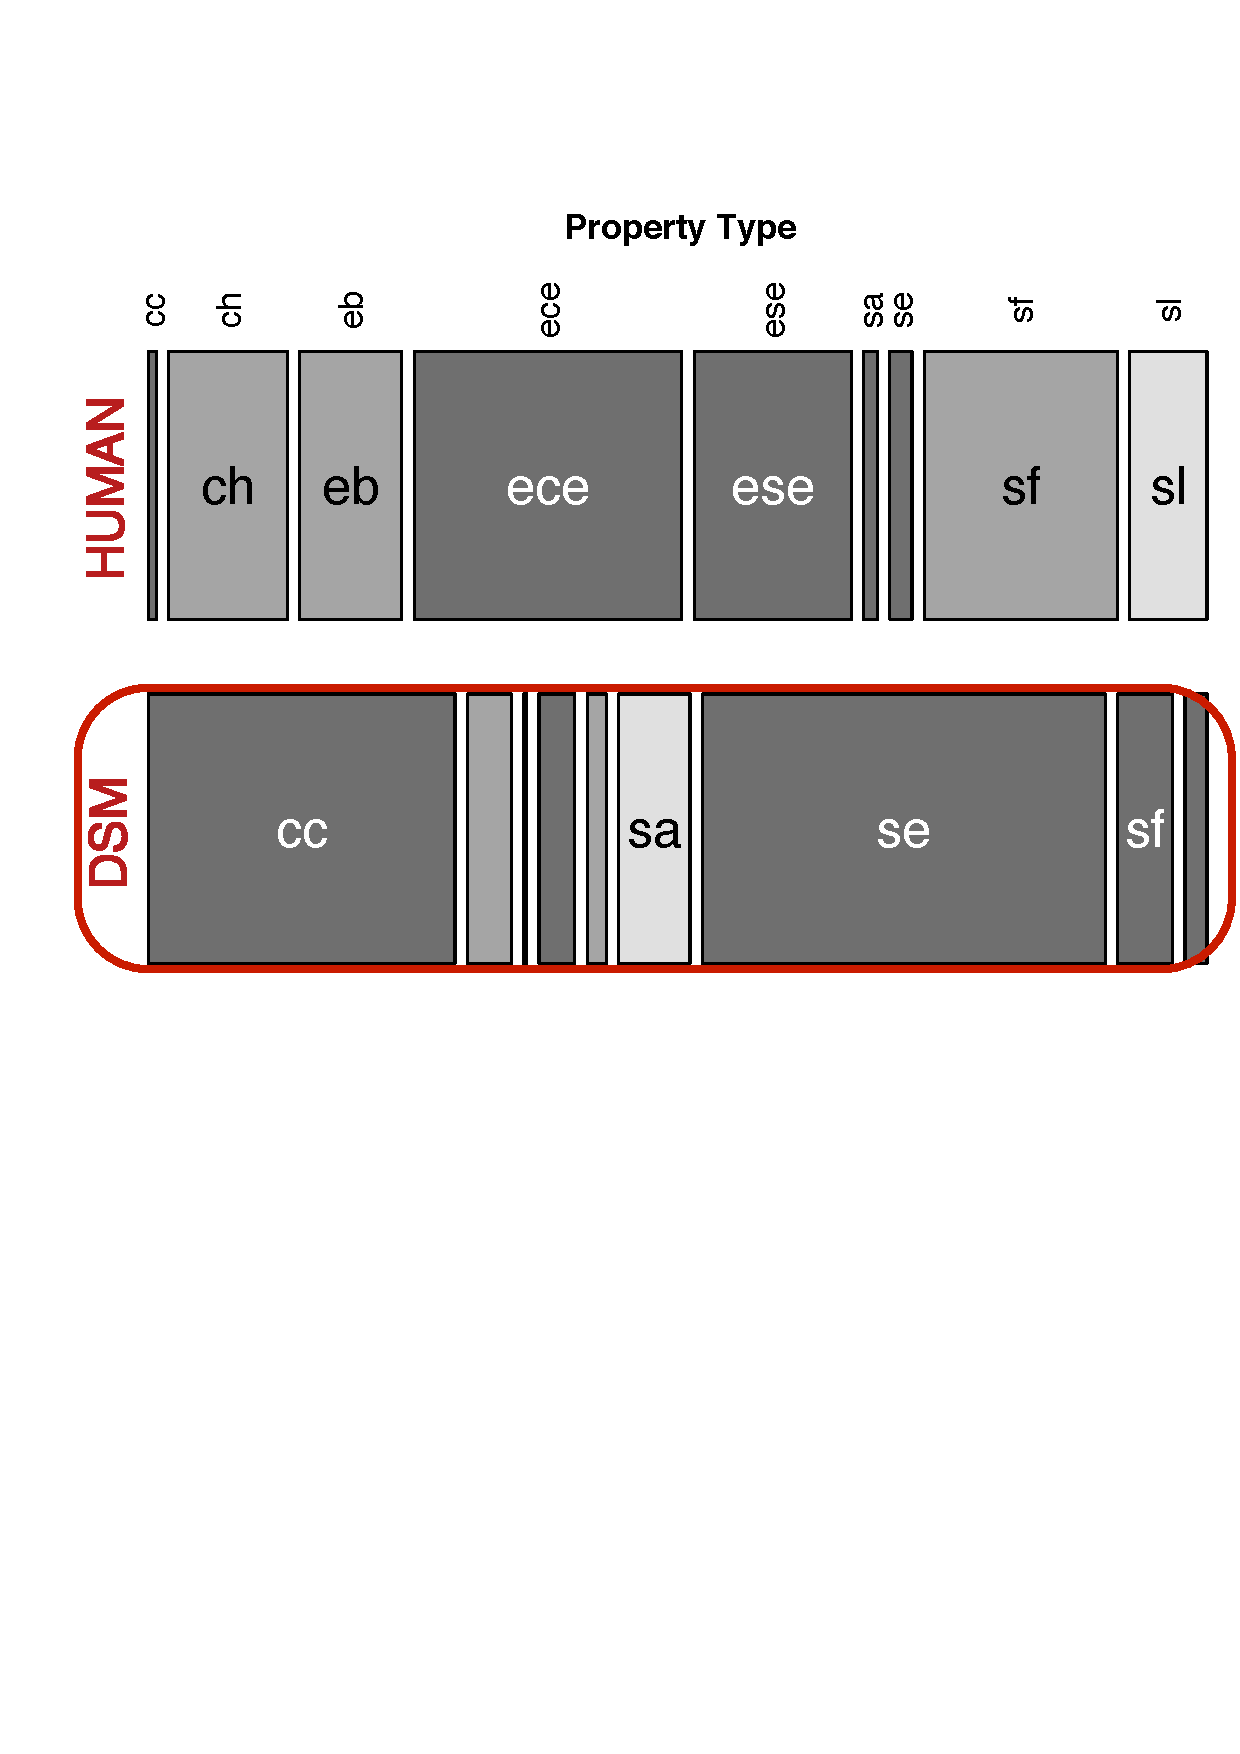
\includegraphics[width=7cm]{img/BaroniLenci2008_fig1_reduced}%
    \end{column}
    \begin{column}{4cm}

      \footnotesize
      Taxonomic category:
      \begin{itemize}\setlength{\itemsep}{0pt}\setlength{\parskip}{0pt}\vspace{-\topsep}
      \item[cc] (co-)hyponym \hfill \textit{truck}
      \item[ch] hypernym  \hfill  \textit{vehicle}
      \end{itemize}
      Properties of entity:
      \begin{itemize}\setlength{\itemsep}{0pt}\setlength{\parskip}{0pt}\vspace{-\topsep}
      \item[eb] typical behaviour  \hfill 
      \item[ece] ext. component  \hfill wheel
      \item[ese] surf. property  \hfill smooth
      \end{itemize}
      Situationally associated:
      \begin{itemize}\setlength{\itemsep}{0pt}\setlength{\parskip}{0pt}\vspace{-\topsep}
      \item[sa] action  \hfill  \textit{park}
      \item[se] other entity  \hfill  \textit{traffic light}
      \item[sf] function \hfill  \textit{drive}
      \item[sl] location  \hfill  \textit{garage}
      \item[sp] participant  \hfill  \textit{driver}

      \end{itemize}
    \end{column}
  \end{columns}

  \footnotesize\gap[2]
Task: humans: given a word, generate properties; DSM: generate top 10 neighbors. Items: 44 concrete English nouns \citep{Baroni:Lenci:08}.
\end{frame}

\begin{frame}
  \frametitle{DSM similarity: concepts \& terminology}
  \framesubtitle{Attributional similarity \vs semantic relatedness}

  \ungap[1]
  \begin{itemize}
  \item \primary{Attributional similarity} ($\leftarrow$ taxonomic) -- two words sharing a large number of salient features (attributes)
    \begin{itemize}
    \item \secondary{synonymy} (\emph{car/automobile})
    \item \secondary{co-hyponymy} (\emph{car/van/truck})
    \item \secondary{hyperonymy} (\emph{car/vehicle)}\\
      \hand{} subset \so distributional inclusion \citep{LenciBenotto:12}
    \item \secondary{antonymy} (\emph{hot/cold})\\
      \hand{} intuitively they are the opposite of similar, and yet \ldots
    \item[]
    \end{itemize}
  \item<2-> \primary{Semantic relatedness} \citep{Budanitsky:Hirst:06} -- two words semantically associated without necessarily being similar
    \begin{itemize}
    \item \secondary{function} (\emph{car/drive})
    \item \secondary{meronymy} (\emph{car/tyre})
    \item \secondary{location} (\emph{car/road})
    \item \secondary{attribute} (\emph{car/fast})
    \end{itemize}
  \item<2->[\hand] Why similar in DSMs? \visible<3->{co-occur \so overlapping context spans}
  \end{itemize}
\end{frame}


\begin{frame}
  \frametitle{DSM similarity: concepts \& terminology}
  \framesubtitle{Attributional \vs relational similarity}

  \begin{itemize}
  \item \primary{Attributional similarity} ($\leftarrow$ taxonomic) -- two words sharing a large number of salient features (attributes)
    \begin{itemize}
    \item \secondary{synonymy} (\emph{car/automobile})
    \item \secondary{co-hyponymy} (\emph{car/van/truck})
    \item \secondary{hyperonymy} (\emph{car/vehicle)}
    \item[]
    \end{itemize}
  \item \primary{Relational similarity} \citep{Turney:06} -- similar relation between pairs of words (analogy)
    \begin{itemize}
    \item \emph{policeman}$\,:\,$\emph{gun} $\;::\;$ \emph{teacher}$\,:\,$\emph{book}
    \item \emph{mason}$\,:\,$\emph{stone} $\;::\;$ \emph{carpenter}$\,:\,$\emph{wood}
    \item \emph{traffic}$\,:\,$\emph{street} $\;::\;$ \emph{water}$\,:\,$\emph{riverbed}
    \end{itemize}
  \end{itemize}
  \onslide<2->
  \begin{columns}[T]
    \begin{column}{45mm}
      \begin{itemize}
      \item[\hand] Textbook example of neural embeddings application   
      \end{itemize}
    \end{column}
    \begin{column}{50mm}
      \hspace*{-1cm}%
      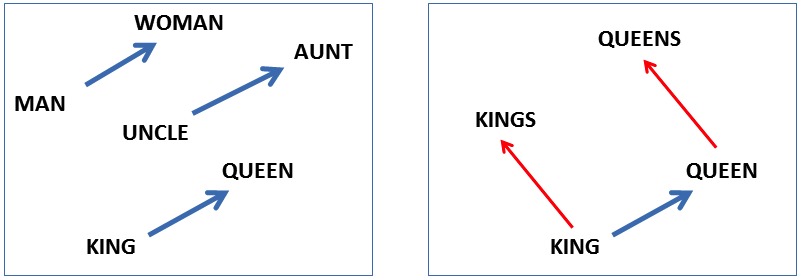
\includegraphics[width=60mm]{img/MikolovYihZweig2013_Fig2}
    \end{column}
  \end{columns}
\end{frame}


\begin{frame}
  \frametitle{Problem: symmetry in DSM similarity}
  \framesubtitle{Symmetric similarity does not fit all phenomena}
  
  \begin{itemize}
  \item Motivation: cognitive processes are notoriously asymmetric\\
    (and so is human intuition about semantic similarity)
  \item Solution: use asymmetric measure of distributional similarity
  \item<2-> Solution: use neighbour rank instead of similarity score
    \begin{itemize}
    \item makes predictions comparable across models and measures
    \item intuition: different density of semantic neighbourhood 
    \item[]
    \end{itemize}
  \end{itemize}

  \onslide<2->
  \begin{minipage}{1\textwidth}
    \hspace{-18pt}
    \begin{minipage}{0.38\textwidth}
      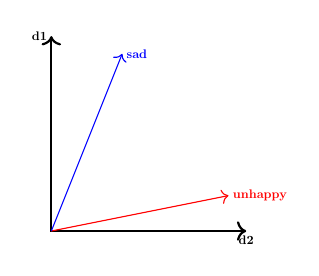
\begin{tikzpicture}[scale=0.45, every node/.style={transform shape}]
        \draw [<->, thick] (0,5.5) -- (0,0) -- (5.5,0);
        \draw [->,red, solid] (0,0) -- (5,1);
        \draw [->,red, blue, solid] (0,0) -- (2,5);
        \node [right,red] at (5,1) {\textbf{unhappy}};
        \node [right,blue] at (2,5) {\textbf{sad}};
        \node [left,black] at (0,5.5) {\textbf{d1}};
        \node [below,black] at (5.5,0) {\textbf{d2}};
      \end{tikzpicture}
      \tiny
      dist(sad, unhappy) = dist(unhappy, sad)
    \end{minipage}
    \onslide<3->
    \begin{minipage}{0.35\textwidth}
      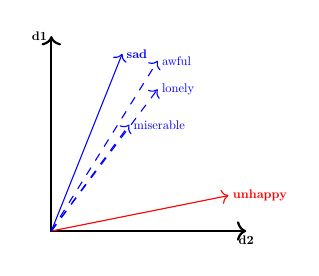
\begin{tikzpicture}[scale=0.45, every node/.style={transform shape}]
        \draw [<->, thick] (0,5.5) -- (0,0) -- (5.5,0);
        \draw [->,red, solid] (0,0) -- (5,1);
        \draw [->,red, blue, solid] (0,0) -- (2,5);
        \draw [->,blue, dashed] (0,0) -- (2.2,3);
        \node [right,blue] at (3,4.8) {awful};
        \draw [->,blue, dashed] (0,0) -- (3,4.8);
        \node [right,blue] at (2.2,3) {miserable};
        \node [right,red] at (5,1) {\textbf{unhappy}};
        \node [right,blue] at (2,5) {\textbf{sad}};
        \node [right,blue] at (3,4) {lonely};
        \draw [->,blue, dashed] (0,0) -- (3,4);xs
        \node [left,black] at (0,5.5) {\textbf{d1}};
        \node [below,black] at (5.5,0) {\textbf{d2}};
      \end{tikzpicture}
      \tiny
      rank(sad, unhappy) =  4
    \end{minipage}
    \begin{minipage}{0.25\textwidth}
      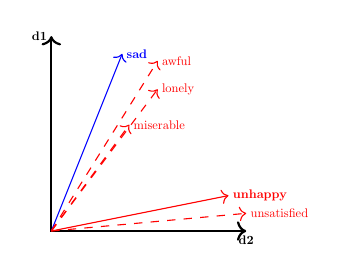
\begin{tikzpicture}[scale=0.45, every node/.style={transform shape}]
        \draw [<->, thick] (0,5.5) -- (0,0) -- (5.5,0);
        \draw [->,red, solid] (0,0) -- (5,1);
        \draw [->,red, blue, solid] (0,0) -- (2,5);
        \node [right,red] at (5,1) {\textbf{unhappy}};
        \node [right,red] at (5.5, 0.5) {unsatisfied};
        \draw [->,red, dashed] (0,0) -- (5.5, 0.5);
        \draw [->,red, dashed] (0,0) -- (2.2,3);
        \node [right,red] at (3,4) {lonely};
        \draw [->,red, dashed] (0,0) -- (3,4);
        \node [right,red] at (2.2,3) {miserable};
        \node [right,red] at (3,4.8) {awful};
        \draw [->,red, dashed] (0,0) -- (3,4.8);
        \node [right,blue] at (2,5) {\textbf{sad}};
        \node [left,black] at (0,5.5) {\textbf{d1}};
        \node [below,black] at (5.5,0) {\textbf{d2}};
      \end{tikzpicture}
      \tiny
      rank(unhappy, sad) =  5
    \end{minipage}
  \end{minipage}
\end{frame}


%%%%%%%%%%%%%%%%%%%%%%%%%%%%%%%%%%%%%%%%%% 
\subsection{Three famous examples}

\begin{frame}
  \frametitle{Latent Semantic Analysis \citep{Landauer:Dumais:97}}
  % \framesubtitle{}

  \begin{itemize}
  \item Corpus: 30,473 articles from Grolier's \emph{Academic American Encyclopedia} (4.6 million words in total)
    \begin{itemize}
    \item[\hand] articles were limited to first 2,000 characters
    \end{itemize}
  \item Word-article frequency matrix for 60,768 words
    \begin{itemize}
    \item row vector shows frequency of word in each article
    \end{itemize}
  \item Logarithmic frequencies scaled by word entropy
  \item Reduced to 300 dim.\ by singular value decomposition (SVD)
    \begin{itemize}
    \item borrowed from LSI \citep{Dumais:etc:88}
    \item[\hand] central claim: SVD reveals latent semantic features,\\
      not just a data reduction technique
    \end{itemize}
  \item Evaluated on TOEFL synonym test (80 items)
    \begin{itemize}
    \item LSA model achieved 64.4\% correct answers
    \item also simulation of learning rate based on TOEFL results
    \end{itemize}
  \end{itemize}
\end{frame}

\begin{frame}
  \frametitle{Word Space \citep{Schuetze:92,Schuetze:93,Schuetze:98}}
  % \framesubtitle{}

  \begin{itemize}
  \item Corpus: $\approx 60$ million words of news messages
    \begin{itemize}
    \item from the \emph{New York Times} News Service
    \end{itemize}
  \item Word-word co-occurrence matrix
    \begin{itemize}
    \item 20,000 target words \& 2,000 context words as features
    \item row vector records how often each context word occurs close
      to the target word (co-occurrence)
    \item co-occurrence window: left/right 50 words \citep{Schuetze:98}\\
      or $\approx 1000$ characters \citep{Schuetze:92}
    \end{itemize}
  \item Rows weighted by inverse document frequency (tf.idf)
  \item Context vector = centroid of word vectors (bag-of-words)
    \begin{itemize}
    \item[\hand] goal: determine ``meaning'' of a context
    \end{itemize}
  \item Reduced to 100 SVD dimensions (mainly for efficiency)
  \item Evaluated on unsupervised word sense induction by clustering
    of context vectors (for an ambiguous word)
    \begin{itemize}
    \item induced word senses improve information retrieval performance
    \end{itemize}
  \end{itemize}
\end{frame}

\begin{frame}
  \frametitle{HAL \citep{Lund:Burgess:96}}
  % \framesubtitle{}

  \begin{itemize}
  \item HAL = Hyperspace Analogue to Language
  \item Corpus: 160 million words from newsgroup postings
  \item Word-word co-occurrence matrix
    \begin{itemize}
    \item same 70,000 words used as targets and features
    \item co-occurrence window of 1 -- 10 words
    \end{itemize}
  \item Separate counts for left and right co-occurrence
    \begin{itemize}
    \item i.e.\ the context is \emph{structured}
    \end{itemize}
  \item In later work, co-occurrences are weighted by (inverse) distance \citep{Li:Burgess:Lund:00}
    \begin{itemize}
      \item but no dimensionality reduction
    \end{itemize}
  \item Applications include construction of semantic vocabulary maps
    by multidimensional scaling to 2 dimensions
  \end{itemize}
\end{frame}

\begin{frame}
  \frametitle{HAL \citep{Lund:Burgess:96}}
  % \framesubtitle{}

  \begin{center}
    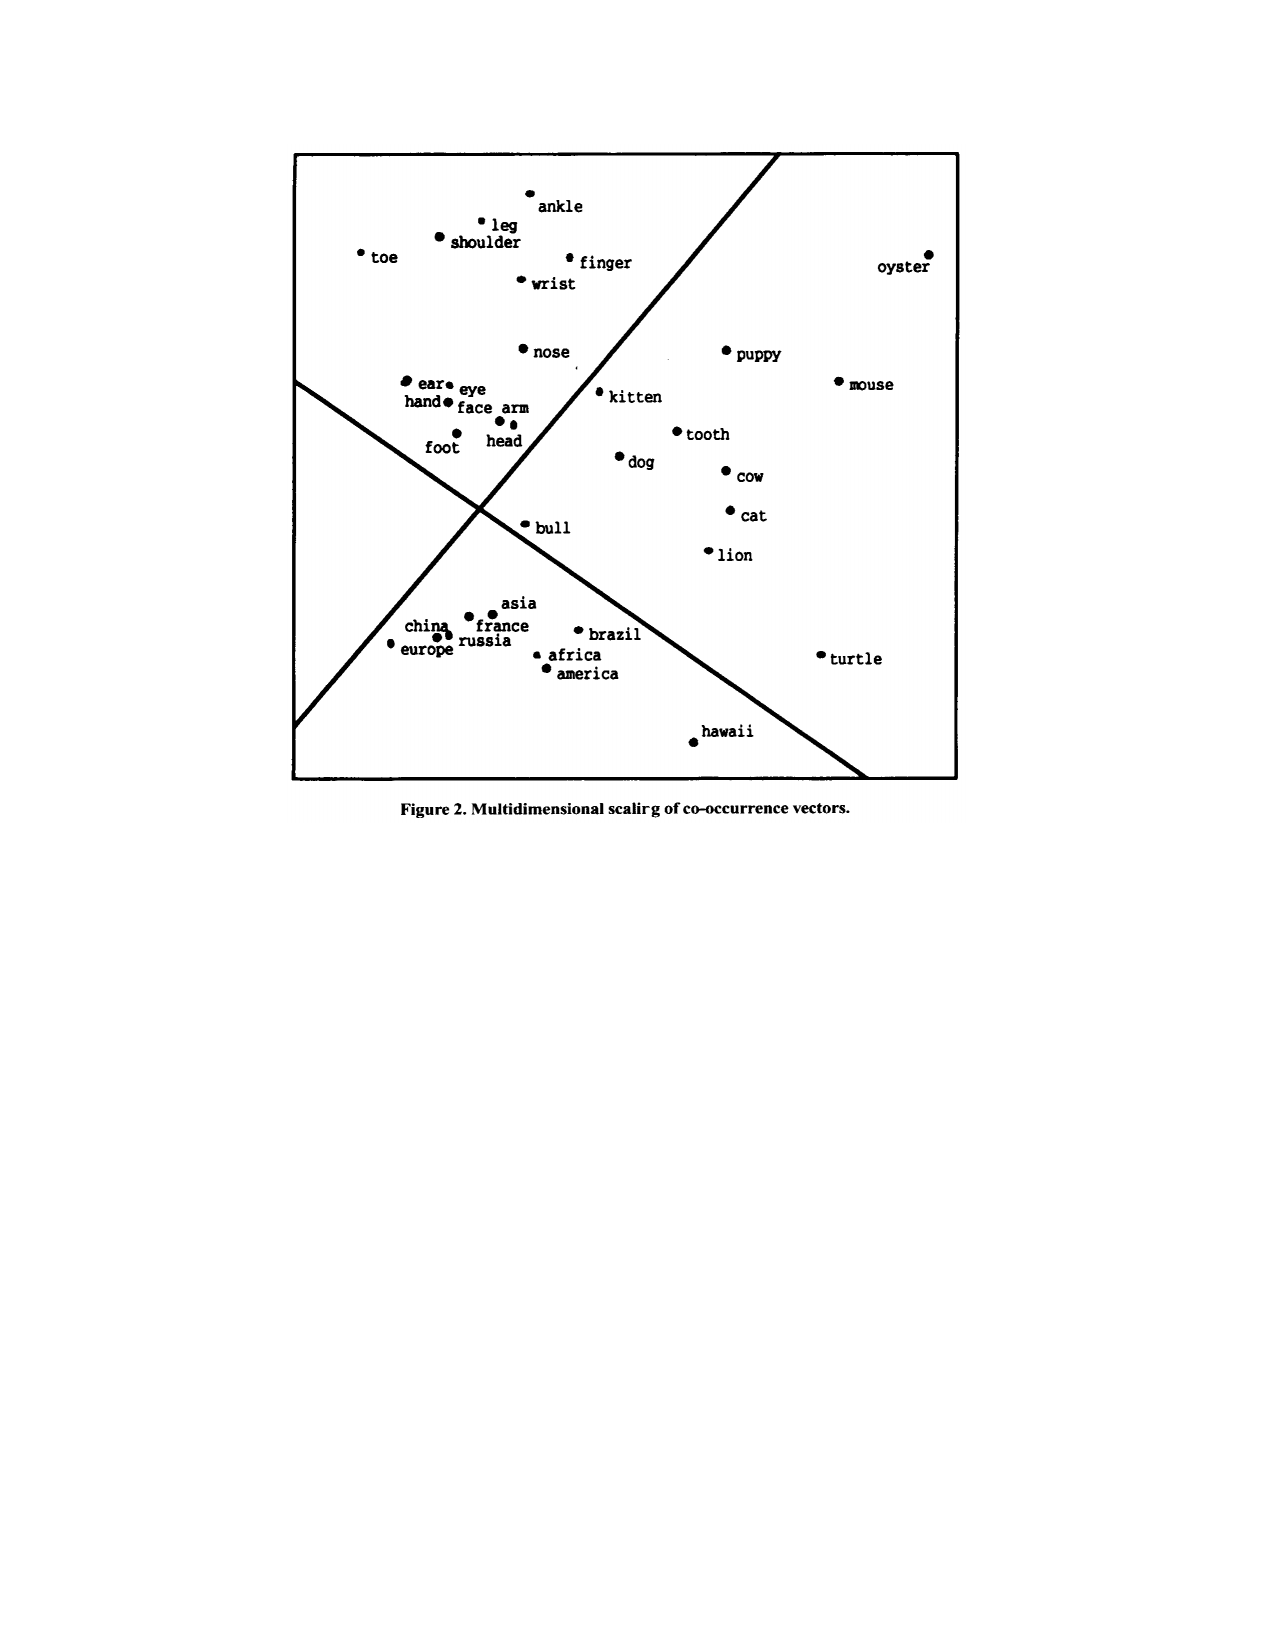
\includegraphics[width=7cm]{img/LundBurgess1996_semantic_map}
  \end{center}
\end{frame}

\begin{frame}
  \frametitle{word2vec embeddings \citep{Mikolov:etc:13b,Mikolov:etc:13}}

  \begin{itemize}
  \item Embeddings are learned by a (simple) neural model rather than obtained directly as distributional vectors
    \begin{itemize}
    \item known as \secondary{predict} rather than \secondary{count} models \citep{Baroni:Dinu:Kruszewski:14}
    \end{itemize}
  \item Corpus: Google News, 6 billion words
  \item Learning objective of the skip-gram model (SGNS)
    \begin{itemize}
    \item predict conditional probability distribution $\pC{c}{t}$ for collocational profile of target word $t$
    \item based on learned target embeddings $\vw_t$ and (ephemeral) collocate embeddings $\vv_c$
    \item[\hand] can be understood as factorisation of co-occurrence matrix \citep{Levy:Goldberg:14,Pennington:Socher:Manning:14}
    \end{itemize}
  \item Evaluation focuses on syntactic and semantic analogy tasks
  \end{itemize}
\end{frame}

\begin{frame}
  \frametitle{Many parameters \ldots}
  % \framesubtitle{}

  \begin{itemize}
  \item Enormous range of DSM parameters and applications
  \item Examples showed four entirely different models, each tuned to its particular application
  \item[]
  \item<2->[\So] Need overview of DSM parameters \& understand their effects
    \begin{itemize}
    \item part 2: The parameters of a DSM
    \item part 3: Evaluating DSM representations
    \item part 4: Understanding distributional semantics
    \item part 5: Mathematical foundations (matrix algebra)
    \item[]
    \end{itemize}
  \item<3->[\So] Distributional semantics is an empirical science
  \end{itemize}
\end{frame}


%%%%%%%%%%%%%%%%%%%%%%%%%%%%%%%%%%%%%%%%%%%%%%%%%%%%%%%%%%%%%%%%%%%%%%
\section{Getting practical}

%%%%%%%%%%%%%%%%%%%%%%%%%%%%%%%%%%%%%%%%%%
\subsection{Software and further information}

\begin{frame}
  \frametitle{Some applications in computational linguistics}
  % \framesubtitle{}

  \ungap[1.5]
  \begin{itemize}
  \item Query expansion in information retrieval \citep{Grefenstette:94}
  \item Unsupervised part-of-speech induction \citep{Schuetze:95}
  \item Word sense disambiguation \citep{Schuetze:98,Rapp:04b}
  \item Thesaurus compilation \citep{Lin:98b,Rapp:04a}
  \item Attachment disambiguation \citep*{Pantel:Lin:00}
  \item Probabilistic language models \citep{Bengio:etc:03b}
  \item Translation equivalents \citep{Sahlgren:Karlgren:05}
  \item Ontology \& wordnet expansion \citep{Pantel:etc:09}
  \item Language change \citep{Sagi:Kaufmann:Clark:09,Hamilton:Leskovec:Jurafsky:16}
  \item Multiword expressions \citep{Kiela:Clark:13}
  \item Analogies \citep{Turney:13,Gladkova:Drozd:Matsuoka:16}
  \item Sentiment analysis \citep{Rothe:Schuetze:16,Yu:etc:17}
  \item[\hand] Input representation for neural networks \& machine learning
  \end{itemize}
\end{frame}

%\begin{frame}
%  \frametitle{Recent workshops and tutorials}
%  % \framesubtitle{}
%
%  \ungap[1]
%  \begin{itemize}
%  \item \primary{2007}: \href{http://clic.cimec.unitn.it/marco/beyond_words/}{CoSMo Workshop} (at Context '07)
%  \item \primary{2008}: \href{http://wordspace.collocations.de/doku.php/workshop:esslli:start}{ESSLLI Wshp} \& \href{http://wordspace.collocations.de/doku.php/workshop:esslli:task}{Shared Task}, \href{http://linguistica.sns.it/RdL/2008.html}{Italian J of Linguistics}
%  \item \primary{2009}: \href{http://art.uniroma2.it/gems/}{GeMS Wshp} (EACL), \href{http://www.let.rug.nl/disco2009/}{DiSCo Wshp} (CogSci), \href{http://wordspace.collocations.de/doku.php/course:esslli2009:start}{ESSLLI}
%  \item \primary{2010}: \href{http://art.uniroma2.it/gems010/}{2nd GeMS} (ACL), \href{http://clic.cimec.unitn.it/roberto/ESSLLI10-dsm-workshop/}{ESSLLI Wshp}, \href{http://naaclhlt2010.isi.edu/tutorials/t4.html}{Tutorial} (NAACL),\\
%   \hide{2010:} \href{https://www.cambridge.org/core/journals/natural-language-engineering/issue/0C6E78AFDAB2AC263CDC331193B5E83A}{J Natural Language Engineering}
% \item \primary{2011}: \href{https://www.aclweb.org/anthology/W/W11/\#1300}{2nd DiSCo} (ACL), \href{https://sites.google.com/site/geometricalmodels/}{3rd GeMS} (EMNLP)
%   %% DiSCo website seems offline: http://disco2011.fzi.de
%  \item \primary{2012}: \href{http://didas.org}{DiDaS Wshp} (ICSC), \href{https://www.cl.cam.ac.uk/~ah433/esslli2012/coursecontent.html}{ESSLLI Course}
%  \item \primary{2013}: \href{https://sites.google.com/site/cvscworkshop/}{CVSC Wshp} (ACL), \href{http://clic.cimec.unitn.it/roberto/IWCS-TFDS2013/}{TFDS Wshp} (IWCS), \href{http://www.dagstuhl.de/en/program/calendar/semhp/?semnr=13462}{Dagstuhl}
%  \item \primary{2014}: \href{https://sites.google.com/site/cvscworkshop2014/}{2nd CVSC} (EACL), \href{https://sites.google.com/site/insightdistsemws/}{DSM Wshp} (Insight)
%  \item \primary{2015}: \href{https://aclanthology.coli.uni-saarland.de/volumes/proceedings-of-the-1st-workshop-on-vector-space-modeling-for-natural-language-processing}{VSM4NLP} (NAACL), \href{https://staff.fnwi.uva.nl/w.zuidema/teaching/compositional-and-vectorial-semantics-esslli-2015/}{ESSLLI Course}, \href{https://hal.archives-ouvertes.fr/hal-01259695/}{TAL Journal}
%  \item \primary{2016}: \href{http://esslli2016.unibz.it/?page_id=256}{DSALT Wshp} (ESSLLI), \href{http://coling2016.anlp.jp/tutorials/T1/}{Tutorial} (COLING), \href{https://sites.google.com/site/konvens2016jobimtexttutorial/}{Tutorial}\\
%    \hide{2016:} (Konvens), \href{http://esslli2016.unibz.it/?page_id=242}{ESSLLI Course}, \href{http://www.aclweb.org/anthology/J/J16/\#4000}{Computational Linguistics}
%  \item \primary{2017}: \href{https://www.irit.fr/esslli2017/courses/34}{ESSLLI Course}
%  \item \primary{2018}: \href{http://text-machine.cs.uml.edu/lrec2018_t4/}{Tutorial} (LREC), \href{http://wordspace.collocations.de/doku.php/course:esslli2018:start}{ESSLLI Course\textsubscript{1}} \& \href{http://esslli2018.folli.info/word-vector-space-specialisation/}{Course\textsubscript{2}}
%  \end{itemize}
%  \hfill\light{\small click on Workshop name to open Web page}
%  \addnote{CoSMo = \underline{Co}ntextual Information in \underline{S}emantic Space \underline{M}odels}%
%  \addnote{ESSLLI = European Summer School in Logic, Language and Information}%
%  \addnote{GeMS = \underline{Ge}ometrical \underline{M}odels of Natural Language \underline{S}emantics}%
%  \addnote{DiSCo = \underline{Di}stributional \underline{S}emantics beyond Concrete \underline{Co}ncepts}%
%  \addnote{JNLE = Journal of Natural Language Engineering}%
%  \addnote{DiSCo 2 = \underline{Di}stributional \underline{S}emantics and \underline{Co}mpositionality}%
%  \addnote{DiDaS = Workshop on \underline{Di}stributional \underline{Da}ta \underline{S}emantics}%
%  \addnote{CVSC = \underline{C}ontinuous \underline{V}ector \underline{S}pace Models and their \underline{C}ompositionality}%
%  \addnote{TFDS = Towards a Formal Distributional Semantics}%
%\end{frame}

\begin{frame}
  \frametitle{Software packages}

  \ungap
  \begin{tabular}{>{\color{secondary}}ll>{\itshape}p{6cm}}
    \href{http://infomap-nlp.sourceforge.net/}{Infomap NLP} & C & classical LSA-style DSM \\
    \href{http://www.psych.ualberta.ca/~westburylab/downloads/HiDEx.download.html}{HiDEx} & C++ & re-implementation of the HAL model \citep{Lund:Burgess:96} \\
    \href{http://code.google.com/p/semanticvectors/}{SemanticVectors} & Java & scalable architecture based on random indexing representation \\
    \href{http://github.com/fozziethebeat/S-Space}{S-Space} & Java & complex object-oriented framework \\
    \href{http://ltmaggie.informatik.uni-hamburg.de/jobimtext/}{JoBimText} & Java & UIMA / Hadoop framework \\
    \href{http://radimrehurek.com/gensim/}{Gensim} & Python & complex framework, focus on parallelization and out-of-core algorithms \\
    \href{http://vecto.space/}{Vecto} & Python & framework for count \& predict models \\
    \href{http://clic.cimec.unitn.it/composes/toolkit/}{DISSECT} & Python & user-friendly, designed for research on compositional semantics \\
    \href{http://wordspace.r-forge.r-project.org/}{\color{primary}\texttt{wordspace}} & R & interactive research laboratory, but scales to real-life data sets\\
    \href{http://text2vec.org/}{\texttt{text2vec}} & R & GloVe embeddings \& topic models
  \end{tabular}

  \gap[0.5]
  \hfill\light{\small click on package name to open Web page}
\end{frame}

\begin{frame}
  \frametitle{Further information}
  % \framesubtitle{}

  \begin{itemize}
  \item Handouts \& other materials available from wordspace wiki at
    \begin{center}
      \secondary{\url{http://wordspace.collocations.de/}}
    \end{center}
  \item[]
  \item Tutorial is open source (CC) and can be downloaded from
    \begin{center}\small
      \secondary{\url{http://r-forge.r-project.org/projects/wordspace/}}
    \end{center}

  \end{itemize}

\end{frame}

\begin{frame}
  \frametitle{Further information}
  % \framesubtitle{}

  \begin{itemize}

  \item Review papers on distributional semantics
    \begin{itemize}
    \item\nocite{Turney:Pantel:10}
      Turney, Peter~D. and Pantel, Patrick (2010).
      \primary{From frequency to meaning: Vector space models of semantics.}
      {\em Journal of Artificial Intelligence Research},  37, 141--188.%
    \item\nocite{Erk:12}
      Erk, Katrin (2012).
      \primary{Vector Space Models of Word Meaning and Phrase Meaning: A Survey.}
      {\em Language and Linguistics Compass},  6-1, 635--653.%      
    \item\nocite{Boleda:20}
      Boleda, Gemma (2020).
      \primary{Distributional Semantics and Linguistic Theory.}
      {\em Annual Review of Linguistics},  6-1, 213--234.%
    \item[]
    \end{itemize}

  \item Textbook on distributional semantics
    \begin{itemize}
    \item\nocite{Lenci:Sahlgren:23}
      Lenci, Alessandro and Sahlgren, Magnus (2023).
      \primary{\em Distributional Semantics.}
      Studies in Natural Language Processing. Cambridge University Press, Cambridge.
    \end{itemize}
  \end{itemize}

\end{frame}

%%%%%%%%%%%%%%%%%%%%%%%%%%%%%%%%%%%%%%%%%%
\subsection{R as a (toy) laboratory}

\begin{frame}
  \frametitle{Prepare to get your hands dirty \ldots}
  
  \begin{itemize}
  \item We will use the statistical programming environment \href{http://www.r-project.org/}{\hh{R}} as a toy laboratory in this tutorial
    \begin{itemize}
    \item[\hand] but one that scales to real-life applications
    \item[]
    \end{itemize}
  \end{itemize}

  Software installation
  \begin{itemize}
  \item \h{R} version 4.0 or newer from \url{http://www.r-project.org/}
  \item \hh{RStudio} from \url{http://www.rstudio.com/}
  \item R packages from CRAN (through RStudio menu)
    \begin{itemize}
    \item \hh{\texttt{sparsesvd}}, \hh{\texttt{wordspace}}
    \item recommended: \hh{\texttt{e1071}}, \hh{\texttt{rsparse}}, \hh{\texttt{Rtsne}}, \hh{\texttt{uwot}}
    \item optional: \secondary{\texttt{tm}}, \secondary{\texttt{quanteda}},  \secondary{\texttt{data.table}}, \secondary{\texttt{wordcloud}}, \secondary{\texttt{shiny}}, \secondary{\texttt{spacyr}}, \secondary{\texttt{udpipe}}, \secondary{\texttt{coreNLP}}
    \end{itemize}
  \item Get data sets, precompiled DSMs and \hh{\texttt{wordspaceEval}} package (with some non-public data sets) from\\ \primary{\href{http://wordspace.collocations.de/doku.php/course:material}{http://wordspace.collocations.de/doku.php/course:material}}
  \end{itemize}
\end{frame}

\begin{frame}
  \frametitle{Prepare to get your hands dirty \ldots}
  \framesubtitle{Installing \texttt{wordspace} and  \texttt{wordspaceEval} in RStudio}
  \centering
  \fbox{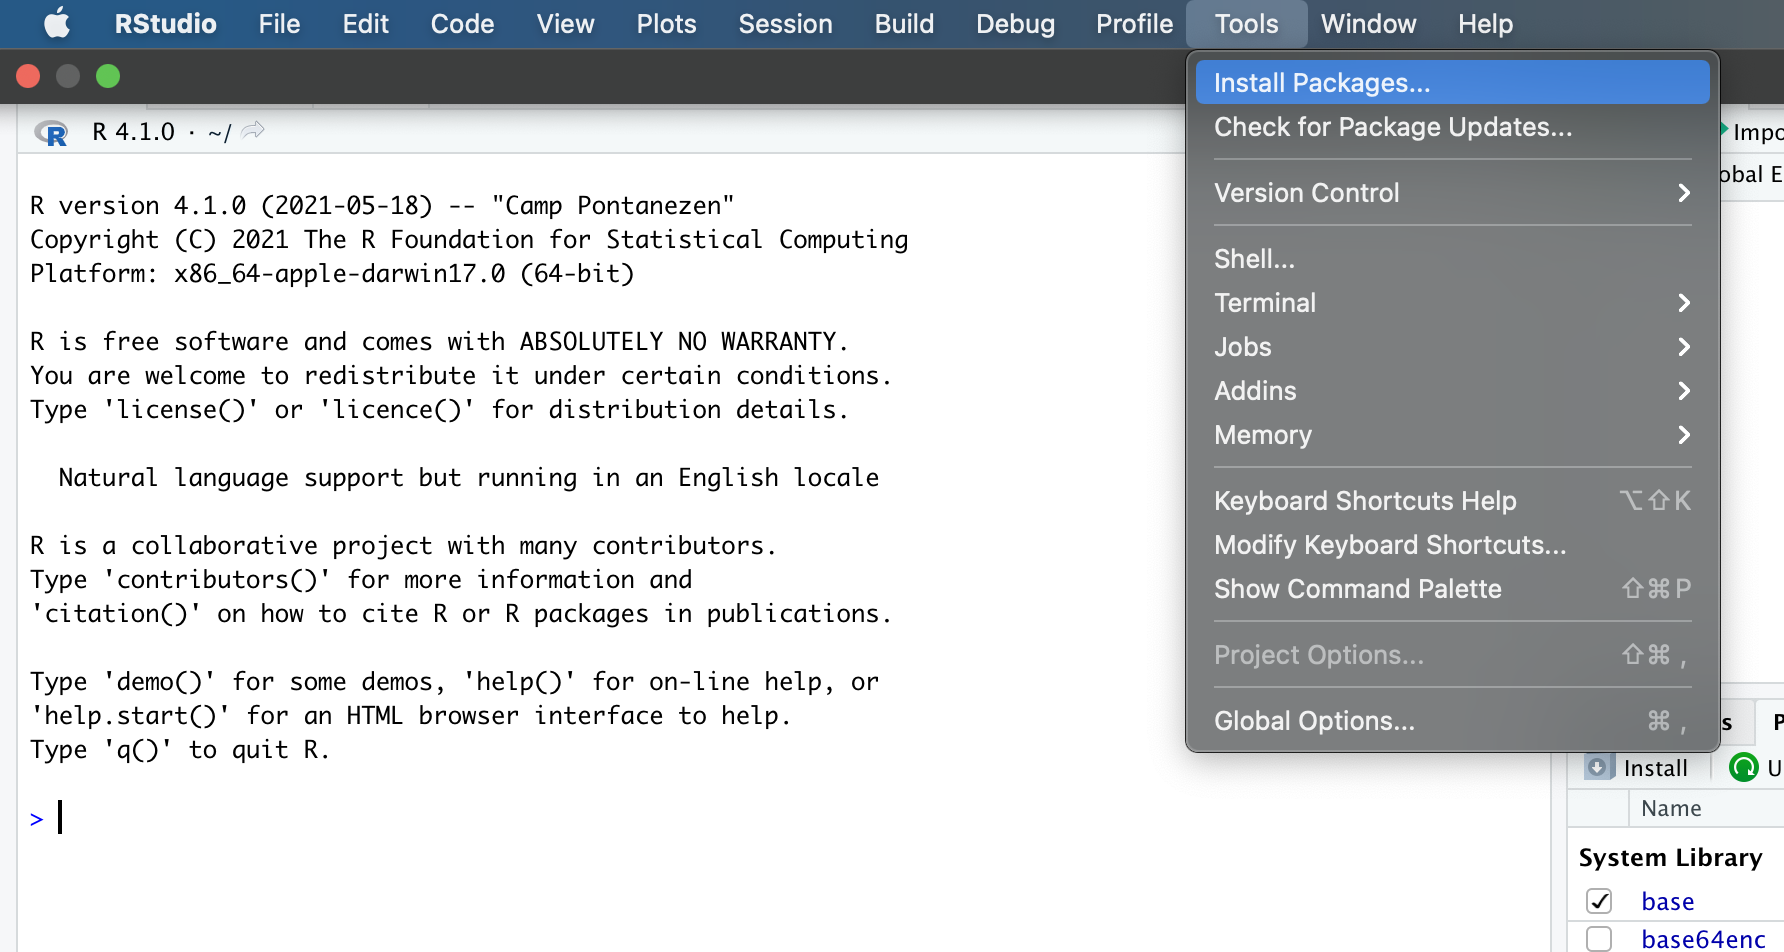
\includegraphics[height=3.5cm]{img/rstudio_install_packages}}  \\
  \bigskip
  \secondary{\scriptsize{\phantom{Eval}\texttt{wordspace}}}
  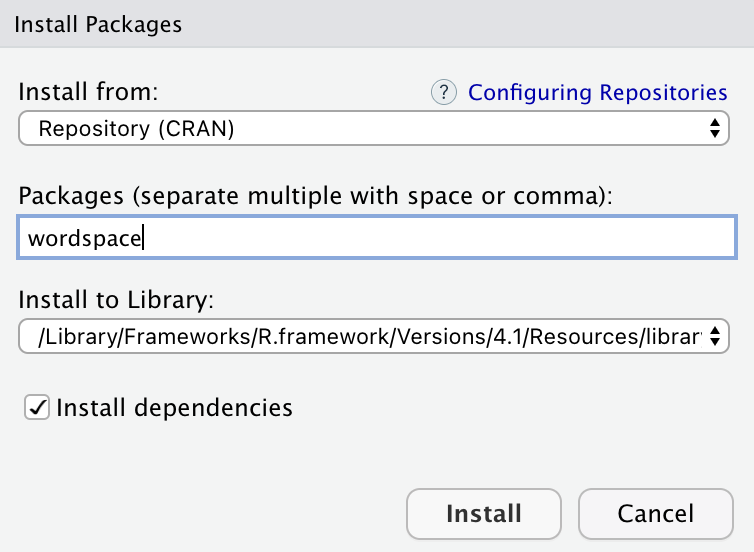
\includegraphics[height=2.2cm]{img/rstudio_install_packages_step1}
  $\;$
  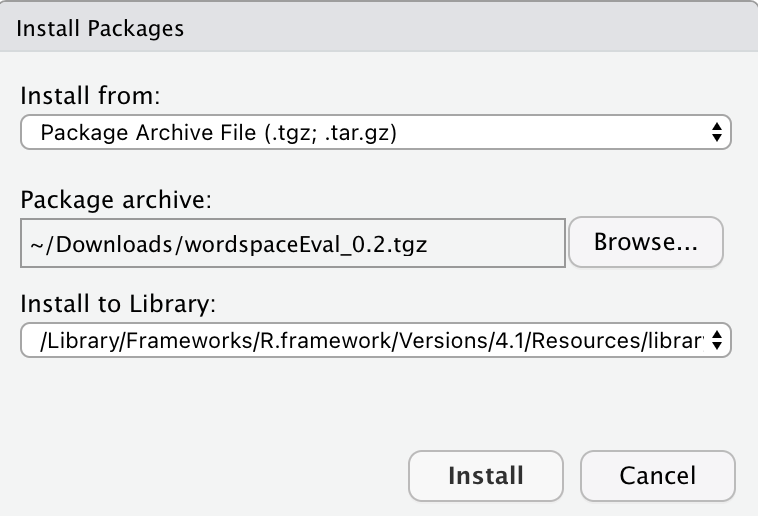
\includegraphics[height=2.2cm]{img/rstudio_install_packages_step2}
  \secondary{\scriptsize{\texttt{wordspaceEval}}}
\end{frame}

\begin{frame}
  \frametitle{Prepare to get your hands dirty \ldots}
  \framesubtitle{Setting up a working directory and RStudio project}

  \begin{itemize}
  \item Create a separate \h{directory} (folder) for this course
    \begin{itemize}
    \item subdirectory \hh{\texttt{models}} for pre-compiled DSMs (large files)
    \item subdirectory \hh{\texttt{data}} for other data files
    \end{itemize}
    \gap
  \item Recommended: set up \h{RStudio project} for the course
    \begin{itemize}
    \item click \emph{New Project} (top right corner), then \emph{Existing Directory}
    \item choose the course directory you've just created
    \item this will be set as your R working directory within the project!
      \itemhand you can easily switch between different RStudio projects
    \end{itemize}
    \gap
  \item Alternatively: set working directory at start of session
    \begin{itemize}
    \item e.g.\ \texttt{setwd("\textasciitilde{}zellig/Desktop/dsm\_tutorial")}
    \end{itemize}
    \gap
  \item Work with \h{R scripts} rather than in interactive console
    \begin{itemize}
    \item RStudio: add \emph{R Script} from drop-down menu in top left corner
    \item we provide example scripts for each part of the tutorial
    \end{itemize}
  \end{itemize}
\end{frame}

\begin{frame}[fragile]
  \frametitle{First steps in R}

  Start each session by loading the wordspace package.
\begin{Rcode}
> library(wordspace)
\end{Rcode}


The package includes various example data sets, some of which should look familiar to you.
\begin{Rcode}
> DSM_HieroglyphsMatrix\begin{Rout}
       get see use hear eat kill
knife   51  20  84    0   3    0
cat     52  58   4    4   6   26
dog    115  83  10   42  33   17
boat    59  39  23    4   0    0
cup     98  14   6    2   1    0
pig     12  17   3    2   9   27
banana  11   2   2    0  18    0
\end{Rout}
\end{Rcode}

\end{frame}

\begin{frame}[fragile]
  \frametitle{Term-term matrix}
  % \framesubtitle{}

  \h{Term-term matrix} records co-occurrence frequencies with feature terms for each target term 
\begin{Rcode}
> DSM_TermTermMatrix
\end{Rcode}

  \gap[2]
  \begin{center}
  \begin{small}
    \setlength{\arrayrulewidth}{1pt}
    \begin{tabular}[c]{r|c@{$\;$}*{6}{|@{$\;$}c@{$\;$}}|}
      \multicolumn{1}{c}{}
      & \multicolumn{1}{c}{\rotLabel{breed}}
      & \multicolumn{1}{c}{\rotLabel{tail}}
      & \multicolumn{1}{c}{\rotLabel{feed}}
      & \multicolumn{1}{c}{\rotLabel{kill}}
      & \multicolumn{1}{c}{\rotLabel{important}}
      & \multicolumn{1}{c}{\rotLabel{explain}}
      & \multicolumn{1}{c}{\rotLabel{likely}} \\
      \cline{2-8}
      cat     &  83 &  17 &   7 &  37 &  -- &   1 &  -- \\
      \cline{2-8}
      dog     & 561 &  13 &  30 &  60 &   1 &   2 &   4 \\
      \cline{2-8}
      animal  &  42 &  10 & 109 & 134 &  13 &   5 &   5 \\
      \cline{2-8}
      time    &  19 &   9 &  29 & 117 &  81 &  34 & 109 \\
      \cline{2-8}
      reason  &   1 &  -- &   2 &  14 &  68 & 140 &  47 \\
      \cline{2-8}
      cause   &  -- &   1 &  -- &   4 &  55 &  34 &  55 \\
      \cline{2-8}
      effect  &  -- &  -- &   1 &   6 &  60 &  35 &  17 \\
      \cline{2-8}
    \end{tabular}
  \end{small}
  \end{center}
\end{frame}


\begin{frame}[fragile]
  \frametitle{Term-context matrix}
  % \framesubtitle{}

  \h{Term-context matrix} records frequency of term in each individual context (e.g.\ sentence, document, Web page, encyclopaedia article)
\begin{Rcode}
> DSM_TermContextMatrix
\end{Rcode}
  
  \gap[2]
  \begin{center}
  \begin{small}
    \setlength{\arrayrulewidth}{1pt}
    \begin{tabular}[c]{r*{7}{|c}|}
      \multicolumn{1}{c}{}
      & \multicolumn{1}{c}{\rotLabel{Felidae}}
      & \multicolumn{1}{c}{\rotLabel{Pet}}
      & \multicolumn{1}{c}{\rotLabel{Feral}}
      & \multicolumn{1}{c}{\rotLabel{Bloat}}
      & \multicolumn{1}{c}{\rotLabel{Philosophy}}
      & \multicolumn{1}{c}{\rotLabel{Kant}}
      & \multicolumn{1}{c}{\rotLabel{Back pain}} \\
      \cline{2-8}
      cat      &      10 &  10 &     7 &    -- &         -- &   -- &        -- \\
      \cline{2-8}
      dog      &      -- &  10 &     4 &    11 &         -- &   -- &        -- \\
      \cline{2-8}
      animal   &       2 &  15 &    10 &     2 &         -- &   -- &        -- \\
      \cline{2-8}
      time     &       1 &  -- &    -- &    -- &          2 &    1 &        -- \\
      \cline{2-8}
      reason   &      -- &   1 &    -- &    -- &          1 &    4 &         1 \\
      \cline{2-8}
      cause    &      -- &  -- &    -- &     2 &          1 &    2 &         6 \\
      \cline{2-8}
      effect   &      -- &  -- &    -- &     1 &         -- &    1 &        -- \\
      \cline{2-8}
    \end{tabular}
  \end{small}
  \end{center}

\end{frame}

\begin{frame}[fragile]
  \frametitle{Some basic operations on a DSM matrix}

\begin{Rcode}
\REM{apply log-transformation to de-skew co-occurrence frequencies}
> M <- log2(DSM_HieroglyphsMatrix + 1) \REM{see part 2}
> round(M, 3)

\REM{compute distributional similarity (cosine measure)}
> pair.distances("dog", "cat", M, convert=FALSE)\begin{Rout}
  dog/cat 
0.9610952\end{Rout}

\REM{find nearest neighbours (defaults to angles)}
> nearest.neighbours(M, "dog", n=3)\begin{Rout}
     cat      pig      cup 
16.03458 20.08826 31.77784\end{Rout}

> plot(nearest.neighbours(M, "dog", n=3, dist.matrix=TRUE))
\end{Rcode}

\end{frame}

\begin{frame}[fragile]
  \frametitle{Playing with a larger model}

  \h{Term-term matrix, dimensionality-reduced}, built from Web texts for
  target words in the format \textit{lemma\_POS} (e.g.\ \texttt{banana\_N})
\begin{Rcode}
> DSM_Vectors
> View(DSM_Vectors)
\end{Rcode}

\gap[1]
Let's inspect some nearest neighbors:
\begin{Rcode}
> nearest.neighbours(DSM_Vectors, "banana_N", n=4)\begin{Rout}
   coconut_N  pineapple_N watermelon_N      bean_N  
    10.86118     12.60826     13.35160     13.79671  
\end{Rout}
\end{Rcode}

\begin{Rcode}
> nearest.neighbours(DSM_Vectors, "freedom_N", n=4)\begin{Rout}
     peace_N   morality_N   equality_N conscience_N 
    30.13420     34.18397     34.23418     34.23894
\end{Rout}
\end{Rcode}
\end{frame}
  
\begin{frame}[fragile]
  \frametitle{Playing with a larger model}

  Or create a semantic map for a word we are interested in:
\begin{Rcode}
> plot(nearest.neighbours(DSM_Vectors, "freedom_N", n=20, 
                          dist.matrix=TRUE))
\end{Rcode}

\begin{center}
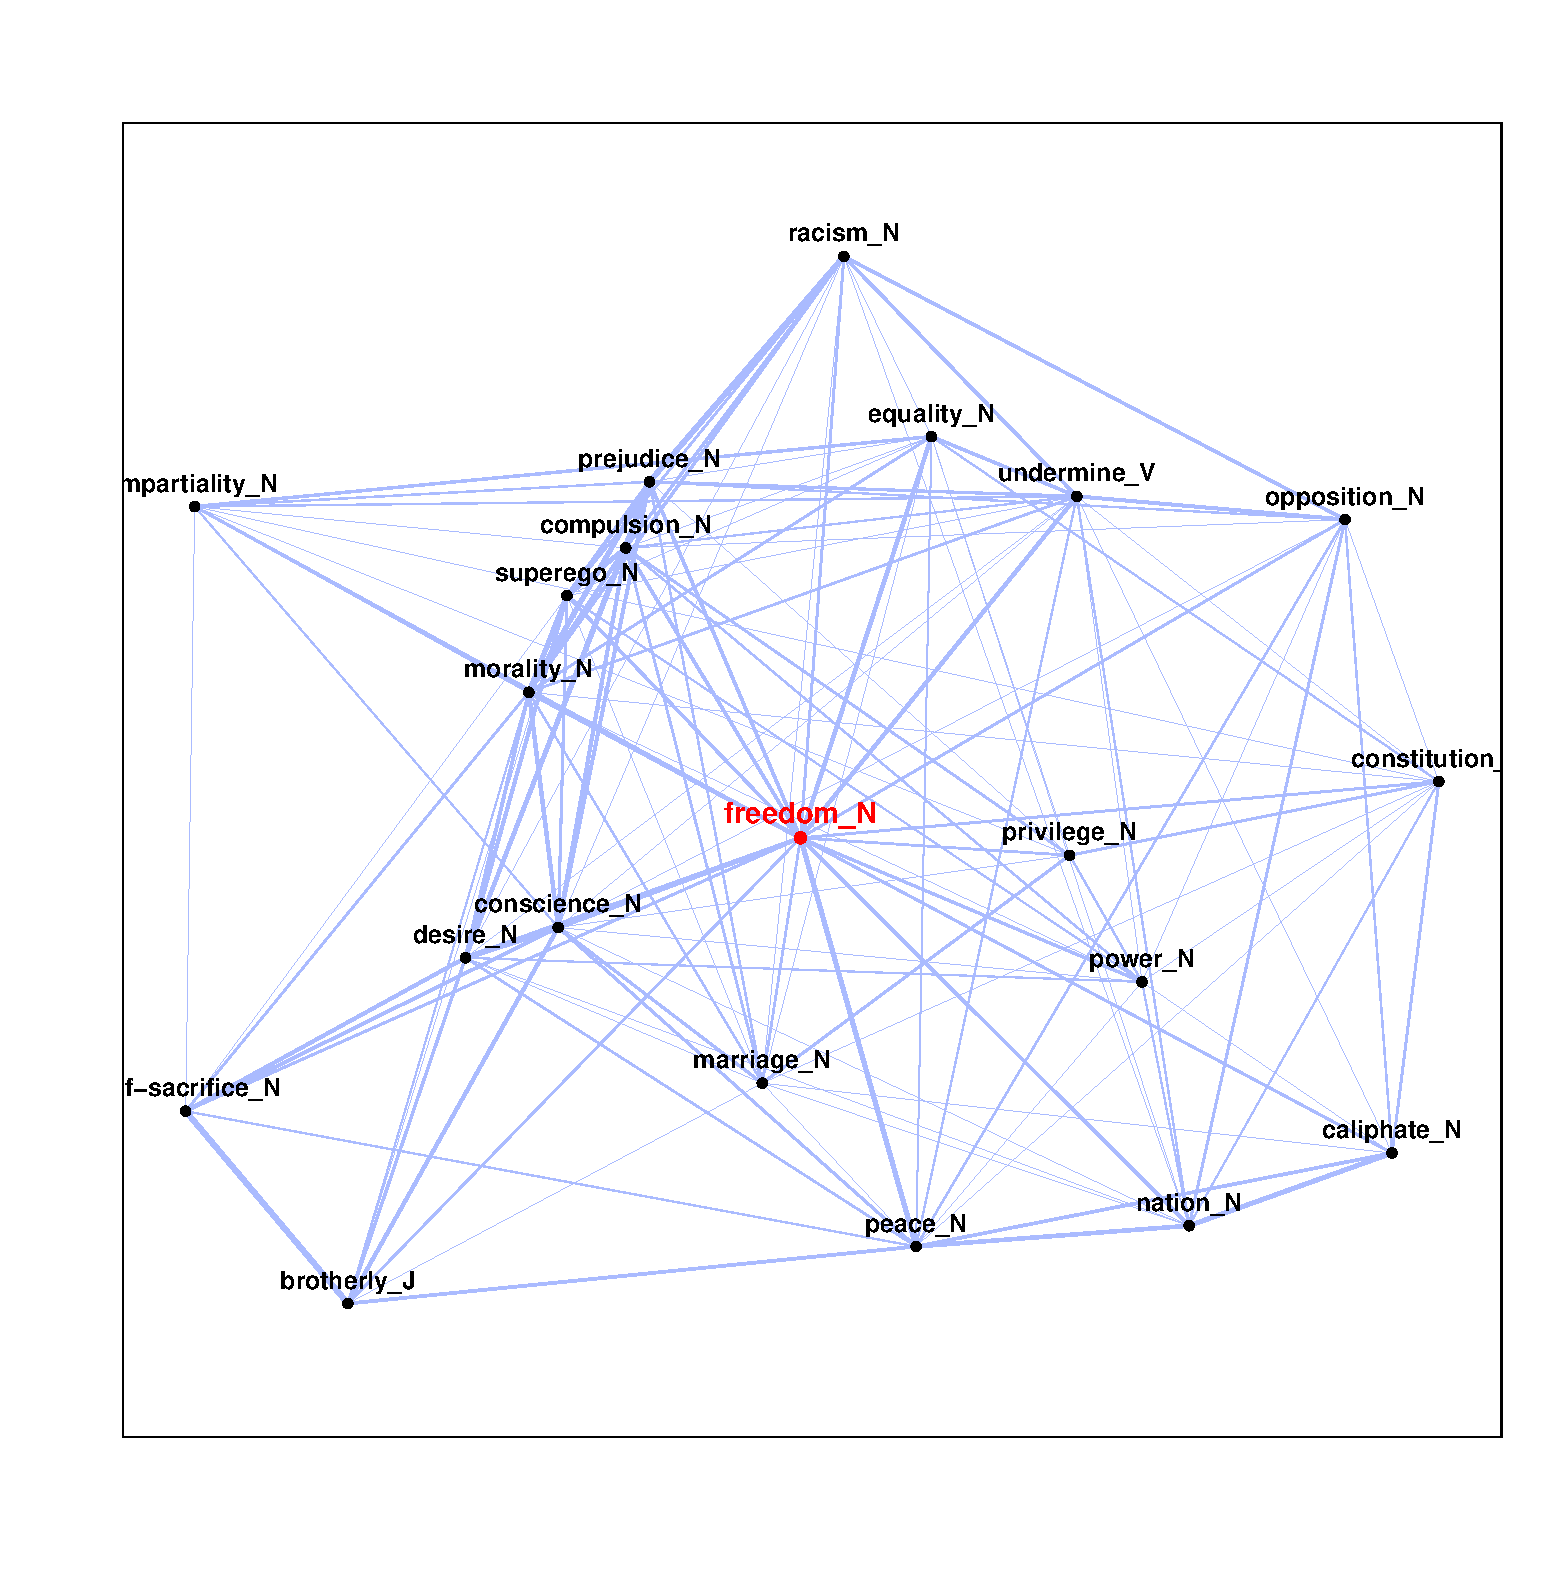
\includegraphics[height=55mm]{img/freedom_DepFilt} 
\end{center}
\end{frame}
  
\begin{frame}[fragile]
  \frametitle{\ldots{} and with an even larger model}

  You can download several \h{large pre-compiled DSMs} from the course wiki, which represent different parameters of the co-occurrence matrix (\so part 2).
  \begin{itemize}
  \item e.g.\ \href{http://corpora.linguistik.uni-erlangen.de/data/wordspace/WP500_DepFilter_Lemma.rda}{\texttt{WP500\_DepFilter\_Lemma.rda}}
  \item download this file to subdirectory \texttt{models}
  \end{itemize}

\begin{Rcode}
> load("models/WP500_DepFilter_Lemma.rda", verbose=TRUE)\begin{Rout}
Loading objects:
  WP500_DepFilter_Lemma
\end{Rout}
> model <- WP500_DepFilter_Lemma \REM{assign to a shorter name}
\end{Rcode}
  
Now try the semantic map again:
\begin{Rcode}
> plot(nearest.neighbours(model, "freedom_N", n=20, 
                          dist.matrix=TRUE))
\end{Rcode}
\end{frame}


\begin{frame}[fragile]
  \frametitle{\textit{Freedom} in a neural embedding model: \texttt{word2vec}}

  \ungap[1]
\begin{Rcode}
> load("GoogleNews300_wf200k.rda", verbose=TRUE)
> embeddings <- GoogleNews300_wf200k.rda
> plot(nearest.neighbours(embeddings, "freedom", n=20, 
                          dist.matrix=TRUE))
\end{Rcode}

\begin{center}
  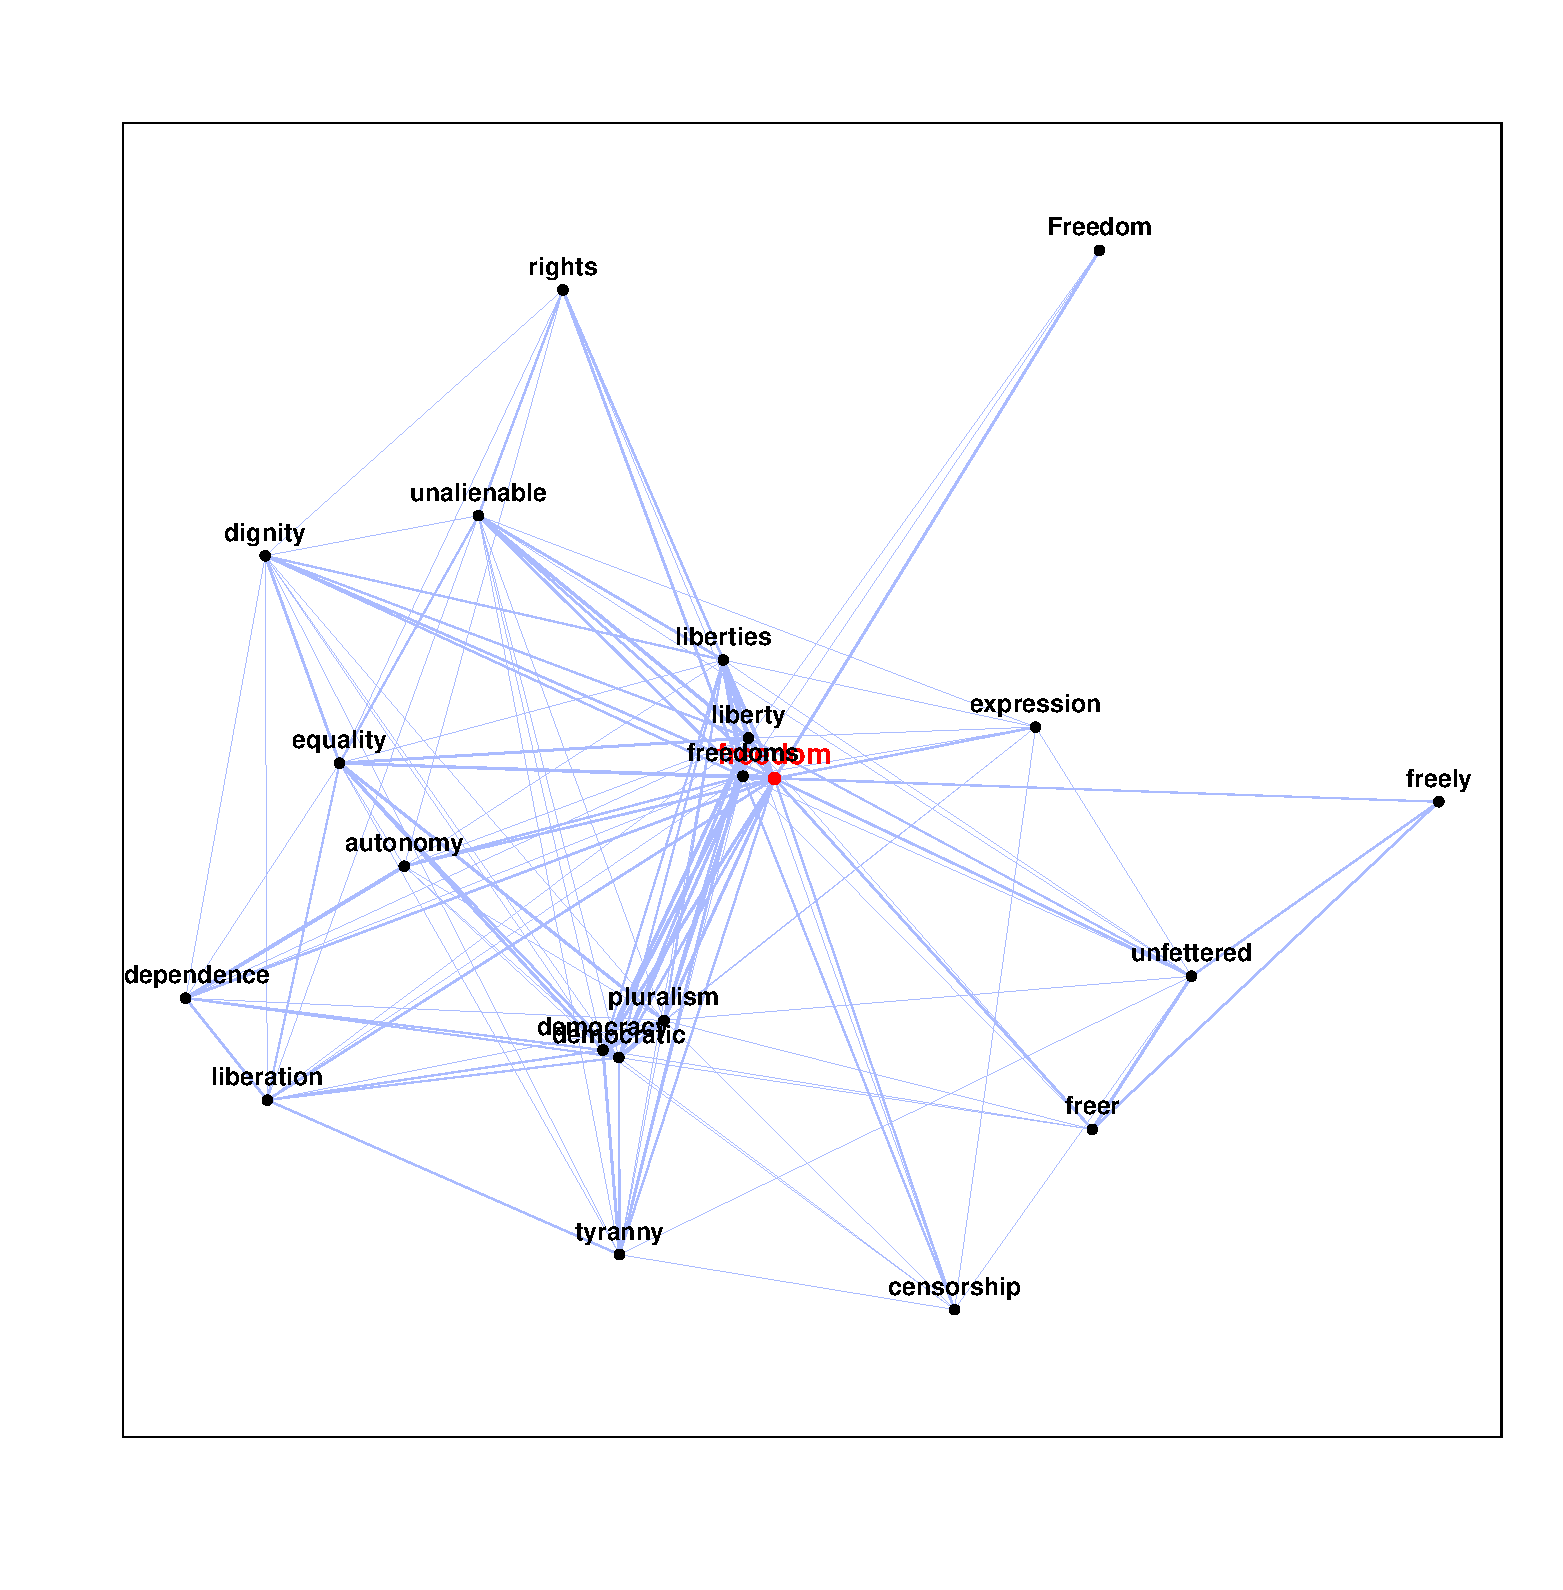
\includegraphics[height=55mm]{img/freedom_w2v}
\end{center}
\end{frame}
  
\begin{frame}[c]
  \frametitle{Explorations}
  
  While you wait for Part 2 of the tutorial,\\ you can explore some DSM similarity networks online:
  \begin{itemize}
  \item \secondary{\href{https://corpora.linguistik.uni-erlangen.de/shiny/wordspace/}{https://corpora.linguistik.uni-erlangen.de/shiny/wordspace/}}
  \item built in R with \texttt{wordspace} and \texttt{shiny}
\end{itemize}
\end{frame}


%%%%%%%%%%%%%%%%%%%%%%%%%%%%%%%%%%%%%%%%%%%%%%%%%%%%%%%%%%%%%%%%%%%%%%
%% References (if any)

\frame[allowframebreaks]{
  \frametitle{References}
  \bibliographystyle{natbib-stefan}
  \begin{scriptsize}
    \bibliography{dsm}
  \end{scriptsize}
}

\end{document}
